\documentclass{article}

\usepackage[spanish]{babel}
\hyphenation{i-rra-dia-dor}
\usepackage[utf8]{inputenc}
\usepackage[backend=bibtex,sorting=none]{biblatex}
\bibliography{bibliografia.bib}
\usepackage{etoolbox}
%\usepackage{todonotes}
%\robustify{\today}
\usepackage[]{hyperref}
%\hypersetup{pdftex,colorlinks=true,allcolors=blue}
\hypersetup{pdfpagemode=UseOutlines}
%\usepackage{hypcap}
\usepackage{amssymb}
\usepackage[]{amsmath}
\usepackage[]{mathrsfs}
\usepackage{graphicx}
\usepackage{float}
\usepackage{caption}
\usepackage{subcaption}
\usepackage[load=addn]{siunitx}
\usepackage{textcomp}

\graphicspath{ {imagenes/} }
\newcommand{\figref}[1]{figura~\ref{#1}}
\newcommand{\equref}[1]{ecuación~\ref{#1}}
% \fig{label}{archivo}{caption}
\newcommand{\fig}[3]{
\begin{figure}[H]
    \centering
    %\includegraphics[width=\columnwidth]{#2}
    \includegraphics{#2}
    \caption{#3}
    \label{fig:#1}
\end{figure}}
\newcommand{\figp}[3]{
\begin{figure}[p]
    \centering
    %\includegraphics[width=\columnwidth]{#2}
    \includegraphics{#2}
    \caption{#3}
    \label{fig:#1}
\end{figure}}
\newcommand{\cita}[1]{\cite{#1}}
\newcommand{\deriv}[2]{\frac{d#1}{d#2}}
\newcommand{\strontium}{\mathrm{Sr}}
\newcommand{\Strontium}{\ensuremath{\left.^{90}\mathrm{Sr}\right.}}
\newcommand{\yttrium}{\mathrm{Y}}
\newcommand{\Yttrium}{\ensuremath{\left.^{90}\mathrm{Y}\right.}}
\newcommand{\zirconium}{\mathrm{Zr}}
\newcommand{\vdd}{\ensuremath{V_{\text{DD}}}}
\def\code#1{\texttt{#1}}

\author{Ignacio Martinez Vazquez}
\date{}

\begin{document}
\tableofcontents
\listoffigures
%
% Está escrita como un informe donde se dice económicamente lo que se hizo.
% A diferencia de un informe, una tesis debe
% -proclamar sus objetivos, en este caso contextualizados por el estado del arte.
% -ir explicando para qué se hace cada cosa (`` a fin de\dots'', ``con el
% propósito de \dots''), y de qué modo se piensa hacer. Y al fin del capítulo con
% los resultados a la vista comparar con lo que se propuso.
% - Hacer una discusión-conclusión-resumen final.
%
% Fijate en algun momento como comparan tus resultados con los pocos
% publicados con estructuras similares, tanto para la tesis como
% pensando en el interés de publicarlos
% pensaba más en los FG de los que tenemos resultados más
% completos, quiero decir carga y descarga eléctrica controladas y
% descarga por radiación medida.
% 
% Respecto de los APS, sí podés ver si lo visto es comparable y tratar
% de tener algun resultado con radiación.
% 
% Otra: Me gustaría que el programa de simulación de la radiación
% (GEANT?) quede instalado en alguna máquina de acá (lo está?) y nos
% ayudes o nos encamines en algunos cálculos. En particular quisiera
% revisar los resultados de Javier que le daba una tasa un poco altísima
% dentro del cañon.
%
\clearpage
\part*{Agradecimientos}
Agradezco a todos los que hicieron posible este trabajo:
\begin{itemize}
    \item Laboratorio de Física de Dispositivos - Microelectrónica: 
    por toda la enseñanza, guía y oportunidades brindadas.
    \item Eriel Fernandez y todo el taller mecánico de FIUBA: 
    por los trabajos y piezas con que aportaron a la construcción del
    irradiador, y por la ayuda en definir los mecanismos.
    \item Abraham Murillo y la Escuela Técnica Nº 33 Fundicion Maestranza del 
    Plumerillo:
    por el planeamiento y realización de la fundición en plomo para el
    irradiador.
    \item Iván G. Pollitzer y el Laboratorio Abierto de Electrónica:
    por la impresión 3D para el irradiador
    \item Universidad de Buenos Aires:
    por la beca estímulo.
    \item CITEDEF: por el wire-bonding de los circuitos fabricados.
\end{itemize}
\clearpage

\section{Introducción}
La radiación es una herramienta con numerosas aplicaciones.

En la industria, se usa para esterilizar instrumental médico y comida,
alterar propiedades químicas de superficies\cite{clough_high},
y para muchos tipos de mediciones.
En particular, se usa para ensayos no destructivos
como la radiografía de neutrones\cite{berger_neutron_1960}.

En medicina, la radiación se emplea en diagnóstico para adquirir imágenes del cuerpo,
y en terapia para tratar cáncer y otras enfermedades.
Con la incidencia creciente de esta enfermedad 
y el uso de radiación en 50\% de los
pacientes\cite{symposium_assurance_dosimetry_1994},
gran parte de la población va a ser expuesta a radiación.

Con el desarrollo de estas aplicaciones,
se empezó a tomar conciencia de 
los peligros de la exposición a la radiación,
y la importancia de entender sus efectos en tejidos
para establecer prácticas seguras.

Una parte central de estas prácticas es el uso de dosímetros personales.
Los mismos permiten limitar los tiempos e intensidades de exposición
por debajo de valores riesgosos.

Además de proteger al personal de un hospital o planta,
los dosímetros permiten monitorear de forma precisa 
el tratamiento que recibe un paciente.
Su uso facilita detectar errores de aplicación\cite{noel_detection_1995}.
También permiten verificar la planificación de nuevas
técnicas y así mejorar el estándar de cuidado\cite{essers_vivo_1999}.
Por último, la dosimetría \emph{in vivo} 
abre la puerta a terapias más efectivas:
es posible planificar cada sesión de radiación
en respuesta al resultado de la anterior,
corrigiendo por fallas de alineamiento, calibración 
y cambios en el paciente\cite{wu_application_2006}.

Este tipo de medición demanda dosímetros 
que se presten al uso médico.
Los requerimientos pasan tanto por sus especificaciones técnicas
(sensibilidad, dosis máxima)
como por su costo,
biocompatibilidad, tamaño,
demora en la lectura y simplicidad de uso.

Desde hace mucho tiempo se usan dosímetros basados en 
dispositivos semiconductores discretos.
Los mismos se basan en el mismo principio que una cámara de ionización de aire,
pero miles de veces más sensibles por unidad de volúmen\cite{jones_application_1963}.
Así posibilitan mediciones con mayor resolución espacial.

Más reciente es un tipo de dosímetro que usa técnicas 
provenientes de la fabricación de circuitos integrados 
para obtener dispositivos 
miniaturizables\cite{holmes-siedle_radfet:_1986}.
Actualmente consisten en circuitos que miden el 
cambio en las características eléctricas de un transistor.
Este es un tipo especial de transistor denominado RADFET,
particularmente sensible a la radiación 
debido a su óxido de compuerta muy grueso.

Dentro de los dosímetros integrables 
(que se pueden incorporar con otras funciones en un circuito integrado),
hay gran interés en aquellos fabricados usando, sin modificación,
procesos comerciales para circuitos integrados\cite{lipovetzky_field_2013}
\cite{wang_temperature_2005}
\cite{garcia-moreno_floating_2012}
\cite{dulinski_cmos_2004}.
Esto elimina la posibilidad de optimizar y controlar 
los parámetros del proceso 
para los requerimientos específicos de dosimetría.
A cambio de esa restricción, 
permite integrar circuitería adicional
para procesamiento de señales e interfaz con el mundo exterior,
y aprovechar las economías de escala de los procesos estándar.

En este trabajo diseñamos, construímos y caracterizamos
dos dosímetros fabricados en un proceso estándar CMOS de
\SI{0.6}{\micro\meter}.
El primero es un Active Pixel Sensor,
de estructura similar a un pixel del sensor de una cámara digital.
El volúmen sensible es la zona desierta de portadores 
de un diodo polarizado en inversa.
La radiación incidente en esta zona genera pares electrón-hueco.
El campo eléctrico separa electrones de huecos y los transporta hacia
terminales opuestas del diodo,
con una fracción de ellos desapareciendo por recombinación.
Así la radiación incidente produce una corriente que va
descargando un capacitor.
El cambio en su valor de carga es un indicador de la energía total recibida.

Su ventaja sobre dosímetros tradicionales es la capacidad de resetearlo
instantáneamente de manera electrónica,
simplemente recargando el capacitor a su valor de carga original.

El segundo dosímetro es un Floating Gate Transistor,
semejante al transistor MOS en una celda de memoria Flash.
Su compuerta se encuentra completamente aislada eléctricamente (flotando),
para almacenar una carga colocada antes de la irradiación.
La radiación incidente genera portadores en el aislante que rodea la compuerta
y va descargándola en proporción a la energía capturada.
Luego de la irradiación,
se mide la carga remanente a través de su efecto en las curvas del transistor.
Este dispositivo es idóneo para dicha medición
porque la corriente que atraviesa la compuerta 
(una fuente indeseada de descarga) es insignificante,
a diferencia de los transistores BJT y JFET.
Este dosímetro se destaca por la posibilidad de medir radiación sin suministro
de tensión, ya que la compuerta flotante retiene su carga durante tiempos muy
largos.

Ambos dosímetros explotan la respuesta a radiación de dispositivos 
normalmente utilizados para otros fines. 
Luego de una introducción a la teoría de su funcionamiento,
presentamos el proceso y las consideraciones de diseño,
y los resultados de las mediciones de ambos dosímetros 
comparando con los valores calculados y cos trabajos previos.

\part{Teoría}
\section{Fundamentals of Metal Oxide Semiconductor structures}
MOS structures are the basis for modern integrated circuits
\cita{sze_physics_2007}
which make up PCs, mobile devices and communication infrastructure.
The CMOS fabrication process which produces these structures
has enabled processing power to grow exponentially,
by steadily shrinking the transistors that make up an integrated circuit
(\figref{fig:moore}).
\fig{moore}{figuras/moore/moore.pdf}
{Exponential reduction in transistor size.
The number of transistors in a microprocessor doubles every two years,
following Moore's law
\cite{moore_cramming_2006}.
Reprinted from \cite{sedra_microelectronic_2010}.}
\subsection{MOS capacitor}
Before studying MOS transistors, it is necessary to understand MOS capacitors.
Fabrication begins with a ~\SI{1}{\milli\meter} silicon wafer cut from a monocrystalline ingot.
Its surface is oxidized in order to produce a thin insulating SiO$_2$ layer.
Both this step and subsequent treatment and annealing steps
determine a crucial property of the Si-SiO$_2$ interface:
the surface density of electronic states.
If this number is too large, the device characteristics are negatively impacted:
for example, through higher noise and parameter shifts over time.
The invention that improved interfaces and thus enabled decent MOS transistors
came decades after the MOS was originally patented
\cite{chih-tang_evolution_1988}.

On top of the oxide layer, a conductor (gate) is deposited,
as seen in \figref{fig:cortemos}.
This conductor can be polysilicon (polycrystalline silicon) or,
in recent processes, metal.
\fig{cortemos}{figuras/mos/corte.png}{Cross section of a MOS structure.
Reprinted from~\cite{sze_physics_2007}.}

This structure forms a capacitor, with two conductors separated by a dielectric.
%
\subsubsection{Band structure}
The following analysis assumes a MOS whose dimensions along the wafer
are much larger than the characteristic distance 
across which the electric field varies normal to the wafer.
This allows us to use a 1D model,
neglecting field variations parallel to the wafer.

The ideal MOS band structure is depicted in \figref{fig:bandasmos}.
An ideal MOS has no charge trapped in the oxide nor in the oxide-semiconductor interface.
Therefore, its bands are flat under zero bias.
We will analyze how band position varies with applied bias and with distance from the wafer surface.

When a voltage source (eg. a battery) is connected across the terminals,
it fixes the difference between the Fermi levels of the metal and the semiconductor.
The resulting $E_F$ gradient leads to a current within the MOS which restores equilibrium
(\figref{fig:polarizacionmos}).

%Bajo la condición $V=0$, los niveles de Fermi de metal y
%semiconductor coinciden.
%Para cada material, el nivel de vacío $\phi$ 
%está a una distancia fija del nivel de Fermi.
%En un metal esta distancia se denomina función trabajo.
%En un semiconductor esta cantidad es la suma de la afinidad electrónica $\xi$
%(distancia entre la banda de conducción y el nivel de vacío)
%y 
%Por ejemplo, la función trabajo del aluminio es \SI{4.2}{\volt} y la de una
%oblea dopada tipo P típica es \SI{3.6}{\volt}.
%Cuando coinciden los niveles de Fermi de metal y semiconductor, 
%difiere su potencial eléctrico en \SI{0.6}{\volt}.
%$\phi$ varía de forma contínua entre las terminales,
%curvando las bandas.
%Hace falta aplicar una tensión $V_{fb}=(\phi_m-\phi_s)/e$ 
%para obtener bandas planas (que implican, por Poisson, carga nula).
%
\fig{bandasmos}{figuras/mos/bandas.png}
{Band structure of a MOS capacitor in the flatband condition.
Reprinted from~\cite{sze_physics_2007}.}
\begin{figure}[H]
    \centering
    \begin{subfigure}[b]{.3\textwidth}
        \includegraphics{figuras/mos/acumulacion.png}
        \label{fig:mosacumulacion}
        \caption{Accumulation}
    \end{subfigure}
    \begin{subfigure}[b]{.3\textwidth}
        \includegraphics{figuras/mos/desercion.png}
        \label{fig:mosdesercion}
        \caption{Depletion}
    \end{subfigure}
    \begin{subfigure}[b]{.3\textwidth}
        \includegraphics{figuras/mos/inversion.png}
        \caption{Inversion}
        \label{fig:mosinversion}
    \end{subfigure}
    \caption{Band structure of a MOS under bias, for $V_{fb}=0$.
Reprinted from~\cite{sze_physics_2007}.}
    \label{fig:polarizacionmos}
\end{figure}
%
\subsubsection{Carrier concentration}
In order to model electron and hole concentration in semiconductors,
one starts from the independent electron approximation.
This means considering one-electron levels which are occupied by identical,
non-interacting electrons.
This type of system is described by Fermi-Dirac statistics,
which state that the probability that a level is occupied is given by
\begin{align*}
    f(E) = \left[\exp\left(\frac{E-E_F}{kT}\right)+1\right]^{-1}
\end{align*}
with $E$ the level energy and $E_F$ the fermi level.
$E_F$ is a constant throughout any system in chemical equilibrium,
and can be solved for as a function of the total number of particles.
This is done by inverting the equation $N=\sum_E f(E)$,
with the sum spanning all energy levels.

In order to calculate the average number of carriers in a band,
it is necessary to sum the occupancy of all the energy levels within it.
We can simplify this sum in the non-degenerate case, where
the conduction band is many thermal energies away from the Fermi level:
$|E-E_F| \gg kT$.
This allows us to approximate the Fermi-Dirac distribution using a
Maxwell-Boltzmann distribution:
\begin{align*}
    f(E) \approx \exp\left(-\frac{E-E_F}{kT}\right)
\end{align*}.
Moreover, the sum over energy levels can be approximated by an integral
over energy, leading to the following hole and electron concentrations:
\begin{align*}
    n_c = N_c(T)e^{-\frac{\epsilon_c-E_F}{k_BT}}\\
    p_v = P_v(T)e^{-\frac{E_F-\epsilon_v}{k_BT}}
\end{align*} with $N_c(T)$ y $P_v(T)$ two slowly-varying functions of temperature.

It is helpful to write the carrier concentration as a function of the bulk potential.
This is a distant reference point in the semiconductor, which we use as a reference:
$\psi_p=\phi(x)-\phi(\infty)$,
\begin{align}
    n &= n_0\exp\left(\frac{q\psi_p}{kT}\right)&
    p &= p_0\exp\left(-\frac{q\psi_p}{kT}\right),
    \label{eq:portadores_nodegenerados}
\end{align}
with $n_0$ and $p_0$ the bulk carrier concentrations.
\subsubsection{Doping}
A central part of the fabrication process is the introduction of dopants
which increase the number of holes or electrons in specific regions.
The geometry and dopant concentration of each region define what kinds of devices
can be created in a given process.
For example, a process might be designed for high voltages by using low concentrations
and large separations, which result in large junction breakdown voltages.

One doping technique is called Chemical Vapor Deposition.
It consists of exposing the wafer to a gas such that atoms diffuse from
the gas phase to the wafer.
Another technique is implanting: dopants are ionized and then accelerated
towards the wafer using electric field.
This allows the penetration depth to be controlled by varying the
acceleration energy
\cite{campbell_science_2001}.

The mechanism by which dopants add carriers is by capturing or emitting electrons.
This ionizes the impurity atom.
In order to model this phenomenon,
impurity atoms are modeled as though they were a normal Silicon lattice atom,
and an additional charge depending on its valence number
(+1 for pentavalent impurities like P, -1 for trivalent like B).
This additional charge can form bound electron states.
By using the effective mass equation\cite{datta_quantum_1989},
% FIXME: feo
one can conclude that the binding energy is typically very low.
Therefore, dopant atoms are almost completely ionized under normal temperature ranges.
This is due to the periodic Silicon lattice, which acts in two ways.
First, it is a dielectric which shields the dopant's electric field.
Second, it gives the electron a smaller effective mass,
which lowers the kinetic energy
(and therefore the potential energy, through the Virial theorem)

Typically, a region has more dopants of one kind than the other,
by several orders of magnitude.
It is then said that the holes or the electrons are the majority carrier.
It can also be said that the region is p-type (majority holes)
or n-type (majority electrons).

Under this condition, the majority carrier concentration is approximately equal
to its dopant concentration.
The minority carrier concentration is suppressed due to Le Chatelier's principle,
and is approximately equal to $n_i^2/N_a$ 
with $n_i$ the intrinsic (pure) carrier concentration for the semiconductor,
and $N_a$ the majority doping concentration.

\subsubsection{Charge-voltage relation}
Starting from Poisson's equation for the semiconductor potential $\phi$,
one reaches
\begin{align*}
    \deriv{^2\phi}{x^2} &= \frac e{\epsilon_s}(N_d-N_a+p-n),
\end{align*}
where the right-hand side terms are concentrations of donors, acceptors,
holes and electrons, respectively.

Approximation~\ref{eq:portadores_nodegenerados} is valid for the nondegenerate
condition
$|E_F-E_{c/v}|\gg kT$, 
meaning the Fermi level is several thermal energies away from the band edges.
This leads to a set of equations which we can solve for the electric field:
\begin{align*}
    \mathscr{E}_s &= \pm \frac{\sqrt 2kT}{qL_D}
    F(q\psi_p/kT,n_{p0}/p_{p0})\textnormal{, with}\\
    L_D^2&=\frac{kT\epsilon_s}{p_{p0}q^2}\textnormal{ , and}\\
    F(x,y) &= \sqrt{e^{-x}+x-1+y(e^x-x-1)}.
\end{align*}
Applying Gauss' law leads to the total charge in the semiconductor:
\begin{align*}
    Q_s = -\epsilon_s\mathscr{E}_s.
\end{align*}

We can find the relation between $V_G$ and $\psi_p$ by
using the voltage drop across the gate oxide,
and the continuity of the normal component of the displacement field:
\begin{align}
    V_G &= \psi_s + \mathscr{E}\frac{\epsilon_s}{\epsilon_{ox}}t_{ox}.
    \label{eq:potencial_campo_mos}
\end{align}
This yields the curve in \figref{fig:cargamos},
where one can highlight the operating regions.
%
\subsubsection{MOS capacitor operating regions}
\begin{itemize}
    \item Accumulation:
        When the gate is negatively biased,
        the semiconductor surface acquires additional majority carriers.
    \item Flatband:
        At zero gate voltage, the positive charge from the holes
        (portadores mayoritarios)
        cancels with the negative charge from the acceptor ions,
        leading to $Q=0$. 
    \item Depletion/weak inversion:
        With increasing gate voltage,
        the semiconductor surface is depleted of majority carriers.
        This leaves behind the negative charge from acceptor ions.
    \item Strong inversion:
        When the surface potential crosses $2\psi_B$,
        the surface is filled with minority electrons,
        with a concentration equaling that of majority carriers in the bulk.
        Additional increases in $\psi_s$ result in exponential growth in
        $|Q|$.
        This remains true until the Fermi level gets close to 
        the conduction band edge, which is called degeneracy.
        When this happens, the semiconductor behaves like a metal,
        whose carrier density varies very weakly with potential.
        Before this point is reached,
        charge grows linearly with $V_G$
        because most additional voltage is dropped across the gate oxide.
\end{itemize}
\fig{cargamos}{figuras/mos/carga_vg.pdf}{Charge in a typical MOS
    ($N_A=$\SI{4e15}{\centi\meter^{-3}}) as a function of gate voltage.
In the left of the graph, the Fermi level grows near to the valence band edge.
This breaks the nondegeneracy assumption, meaning that Fermi-Dirac statistics
must be used without approximation.}
%
%
\subsection{MOS transistor}
Transistors are the base of modern electronics.
By modulating one signal with another,
they implement analog operations like amplification and multiplication.
When used with discrete levels (on/off),
they implement the basic logic gates (NOT, AND, etc)
which combine to form a digital circuit.
Their steady improvement has allowed for a growing number of 
digital and analog functions
to be integrated in a single chip.
%
\subsubsection{Modelo circuital}
\label{section:ecuaciones_mos}
El MOSFET o transistor MOS es un dispositivo con 4 terminales:
drain, gate, source y body (\figref{fig:mosfetschem}).
\fig{mosfetschem}{figuras/mos/mosfet.pdf}{Símbolo esquemático del transistor MOS.}
Frecuentemente se conecta source con body, rompiendo la simetría source-drain.
La tensión entre gate y source controla la corriente drain-source.

En la \figref{fig:mosfetoutput} se ven los 3 modos de operación del MOS:
\fig{mosfetoutput}{figuras/mos/output.pdf}{Curvas características de un
transistor MOS típico.}
\begin{itemize}
    \item Corte: Si $V_g<V_T$, no fluye corriente de drain.
        Por eso $V_T$ es denominada la ``tensión umbral''.
        $V_T$ es un parámetro de fabricación que ronda \SI{.3}{\volt} en procesos CMOS
        modernos.
        Un modelo más preciso es que $I_d$ depende exponencialmente de $V_g$.
    \item Triodo: Si $V_g>V_T$ y $V_{ds}<V_g-V_T$, la corriente de drain crece con la
        tensión drain-source siguiendo
        \begin{align*}
            I_D&=\beta_n\frac WL(V_{gs}-V_T-\frac{V_{ds}}2)V_{ds},
        \end{align*}
        con $\beta_n$ un parámetro del proceso y $\frac WL$ la relación de
        aspecto del MOSFET.
    \item Saturación: Si $V_g>V_T$ y $V_{ds}>V_g-V_T$ la corriente se mantiene, a primer
        orden, al valor constante
        \begin{align*}
            I_{Dsat}&=\frac{\beta_n}2\frac WL(V_{gs}-V_T)^2.
        \end{align*}
\end{itemize}
%
\subsubsection{Modelado físico}
El MOSFET de canal n consiste en un capacitor MOS de sustrato p entre dos regiones fuertemente dopadas 
tipo n, 
que forman drain y source (\figref{fig:mosfetestructura}).
Sin tensión de gate no puede fluir corriente entre drain y source porque una de las
junturas p-n (drain-sustrato o source-sustrato) queda polarizada en inversa.

Al polarizar el MOS en inversión se forma junto al óxido de gate 
una capa de electrones libres llamada canal.
Esta región de tipo n conecta drain y source y permite el flujo de corriente.
Al variar la tensión de gate, la variación de carga en el canal modula su
conductividad.
\fig{mosfetestructura}{figuras/mos/mosfet.png}{Estructura del transistor MOS.
Reproducido de~\cite{sze_physics_2007}.}

\section{Radiation}
\label{sec:radiacion}
Radiation is the transport of energy, mediated by different particles.
This thesis deals mainly with photons (X rays) and electrons ($\beta$ rays).
When these particles carry enough energy,
they interact with matter in such a way to cause ionization.
This can lead to damage both in living tissue and in electronic devices.
%
\subsection{$\alpha$ radiation}
$\alpha$ particles are $^4$He nuclei.
They are produced by unstable nuclei such as
$^{241}$Am (which is used in smoke detectors) and U,
in a process known as $\alpha$ decay.
This process can generate particles with energies close to
\SI{5}{\mega\electronvolt},
which are stopped after traveling through a few centimeters of air
or the layer of dead cells on the epidermis.
They are typically not hazardous for humans,
except when inhaled or ingested,
or if they have very high energies (eg. from cosmic rays)
\subsection{Neutrons}
Neutrons are neutral particles which are present in atomic nuclei.
The various isotopes of each element are nuclei which only differ in the number of neutrons.
Nuclear fusion and fission usually emit high-energy neutrons or,
in nucleosynthesis processes,
capture neutrons and thus form heavier nuclei.

For protection purposes, the relevant interactions between neutrons and nuclei
are elastic scattering, inelastic scattering and capture.
In inelastic scattering,
part of the incoming neutron's energy excites the target nuclei to a higher energy level.
This energy is later emitted as photons when the nucleus relaxes.
Capture happens with lower energy neutrons,
for example those which have lost energy to scattering,
and produces $\gamma$ rays
For example, in boron neutron capture therapy,
boron is delivered to cancer cells.
When irradiated with neutrons, these cells are destroyed
by the $\alpha$ and $\gamma$ radiation produced by the capture process.
\subsection{$\beta$ radiation}
$\beta$ radiation consists of high-energy electrons.
These can travel through matter and deposit energy through ionization,
or emit energy as braking radiation (bremsstrahlung)
This limits the range or penetration depth into a material before they run out of energy.
Their range in air is in the order of meters,
while denser materials can restrict their range to millimeters.

Everyday matter is largely composed of electrons (by number).
However, these electrons are bound to atomic nuclei,
and lack the energy to escape the potential well.
When $\beta$ or $\gamma$ radiation strikes a material,
it can produce free electrons (secondary $\beta$ radiation)
if the incoming particle energy exceeds the material ionization energy.

$\beta$ radiation can also be produced by decaying radioactive isotopes,
in a process called $\beta$ decay.
\subsubsection{$\beta$ decay}
$\beta$ decay is a process whereby an atomic nucleus $X$ 
turns into a lighter nucleus $X'$,
emitting an electron and an electron antineutrino.
For example, strontium decaying to Yttrium:
\begin{align*}
    \left.^{90}\strontium\right.
    &\to\left.^{90}\yttrium\right.+e^-+\overline\nu_e.
\end{align*}
The variation in the number of atoms $N_X$ as a function of time follows the equation
\begin{align*}
    \deriv{N_X}t &= -\lambda N_X\\
    \deriv{N_{X'}}t &= \lambda N_X
\end{align*}
if $X'$ is stable over the timescales of interest.
$\lambda$ is a parameter which sets the decay rate.
In the context of radiation, this decay rate is called activity
and is measured in Becquerel (\SI{1}{\becquerel}=\SI{1}{\per\second})
or Curie (1 Ci=\SI{3.7e10}{\per\second}).
The solutions to this equation are of the form
\begin{align}
    \label{eq:soluciondecaimiento}
    N_X(t) &= N_X(0)e^{-\lambda t}\\
    N_{X'}(t) &= N_X(0)(1-e^{-\lambda t}).\nonumber
\end{align}
Rather than $\lambda$, it is more usual to speak of the half life of $X$.
This is the time $\tau$ it takes for $N_X$ to halve.
Its relation to $\lambda$ can be deduced from \equref{eq:soluciondecaimiento}.
\begin{align*}
    \frac 1 2 N_X(0) &= N_X(0)e^{-\lambda\tau}\\
    \tau &= \frac{\ln2}\lambda
\end{align*}
\subsubsection{Secular equilibrium}
The lighter nucleus produced by $\beta$ decay may itself be unstable.
For example, $^{90}\strontium$ decays to $^{90}\yttrium$ 
which in turn decays to $^{90}\zirconium$.
The quantities of each element follow the equations
\begin{align*}
    \deriv{N_\strontium}t &= -\lambda_\strontium N_\strontium\\
    \deriv{N_\yttrium}t &= \lambda_\strontium N_\strontium
        -\lambda_\yttrium N_\yttrium\\
    \deriv{N_\zirconium}t &= \lambda_\yttrium N_\yttrium.
\end{align*}
The solutions are of the form
\begin{align*}
    N_\strontium(t) &= N_\strontium(0)e^{-\lambda_\strontium t}\\
    %\deriv{N_\yttrium}t +\lambda_\yttrium N_\yttrium &= 
        %\lambda_\strontium N_\strontium(0)e^{-\lambda_\strontium t}
    N_\yttrium(t) &= ae^{-\lambda_\yttrium t}
        +N_\strontium(0)\frac{\lambda_\strontium}
        {\lambda_\yttrium-\lambda_\strontium}e^{-\lambda_\strontium t}.
\end{align*}
Because $^{90}\yttrium$'s half life (2.7 days) 
is much smaller than $^{90}\strontium$'s (29 years),
it holds that $\lambda_\yttrium\gg\lambda_\strontium$.
Therefore, the quantities of both elements reach a secular equilibrium given by
\begin{align*}
    N_\strontium(t) &= N_\strontium(0)e^{-\lambda_\strontium t}\\
    N_\yttrium(t) &\approx N_\strontium(0)
        \frac{\lambda_\strontium}{\lambda_\yttrium}
        e^{-\lambda_\strontium t}.
\end{align*}

The activity is
\begin{align*}
    A_\strontium(t) &= N_\strontium(0)\lambda_\strontium
        e^{-\lambda_\strontium t}\\
    A_\yttrium(t) &\approx N_\strontium(0)
        \frac{\lambda_\strontium}{\lambda_\yttrium}\lambda_\yttrium
        e^{-\lambda_\strontium t}=A_\strontium(t).
\end{align*}
Therefore, a $^{90}\strontium$ source in secular equilibrium
owes half of its activity to $\strontium\to\yttrium$ decays
and half to $\yttrium\to\zirconium$ decays.
%
\subsubsection{Electronic stopping}
Electrons lose energy through discrete interactions with the atoms that make up matter.
This series of interactions can be approximated as
a continuous variation of energy with distance $\epsilon(x)$.
This allows us to define a stopping power $S(\epsilon)$ for each material such that
\begin{align*}
    \frac{d\epsilon}{dx}=-S(\epsilon).
\end{align*}

One is typically interested in studying protection from a beam of electrons,
rather than a single electron.
Beams can be characterized by their particle flux (number of particles per unit time)
$\dot N=\frac{dN}{dt}$
or their fluence rate (number of particles per unit time, per unit area)
$\dot\Phi=\frac{dN}{dAdt}$.

In calculating a beam's dose rate (deposited energy per unit time, per unit mass),
one typically works with the mass stopping power $S/\rho$,
which is the stopping power divided by the material density.
This leads to a simple expression for the dose rate:
\begin{align*}
    \dot D&=\deriv{}{t}\deriv{E}{m}=\deriv{\epsilon dN}{mdt}=\frac
    1\rho\deriv{\epsilon}{x}\deriv{N}{Adt}=
    I\frac{S}\rho
\end{align*}
$S$ and $S/\rho$ are tabulated for many elements and materials (\figref{fig:stopping}).
\fig{stopping}{figuras/rad/stopping.pdf}{Electronic stopping power
for different materials as a function of energy.
Values published by NIST's ESTAR project\cite{berger_estar_????}.}
Another tabulated quantity is the range,
which is how far they can travel through a material in a straight line
before exhausting their energy:
\begin{align*}
    R(\epsilon) &= \int_0^\epsilon \frac{d\epsilon'}{S(\epsilon')}
\end{align*}

Finally, there is the radiation yield $Y$.
This is the fraction of energy which is emitted as photons
(braking radiation or bremsstrahlung).
$Y$ is an increasing function of atomic number.
For protection purposes, it is common to stop electrons with
polymers such as acrylic, which have low radiation yield.
This minimizes X ray production,
meaning less lead is required to absorb the braking radiation.
%
\subsection{X radiation}
X rays are photons with wavelengths between \SI{0.03}{\nano\meter} and \SI{10}{\nano\meter}.
They carry sufficient energy to ionize many materials.
They are typically produced when charged particles interact with matter.
\subsubsection{Braking radiation (bremsstrahlung)}
When a charged particle accelerates, it emits electromagnetic radiation
\cite{jackson_classical_1998}.
Bremsstrahlung is an example of this,
produced by electrons which slow down in matter.
It occurs naturally as cosmic rays interact with the atmosphere,
and artificially in X ray tubes as electrons impact a metallic target.

Bremsstrahlung photons have a power spectral density given by
Kramers' law\cite{kramers_xciii._1923}
\begin{align}
    P(E)dE = \frac{2P_T}{E_M^2}(E_M-E)dE
    \label{eq:kramers}
\end{align} with $E_M$ the incoming electron energy (\figref{fig:kramers}).
\fig{kramers}{figuras/rad/kramers.pdf}
{Power spectral density produced by stopping electrons with energy $E_M$,
with total power $P_T$.}
$P_T$ is the total bremsstrahlung power, given by
\begin{align*}
    P_T&=E_MIY(E_M)
\end{align*} with $I$ the electron flux
and $Y$ the radiation yield for the target material at that energy.
\subsubsection{X ray shielding}
We model X ray intensity as a continuous function of energy and position $I(E,x)$.
This allows us to define an absorption coefficient $\mu(E)$ for each material
(\figref{fig:absorcionX}) such that
\fig{absorcionX}{figuras/rad/absorcionX.pdf}
{X ray absorption coefficient $\mu$ as a function of energy.
    Values tabulated by NIST\cite{xraycoef}.}
\begin{align}
    \label{eq:absorcionx}
    dI/dx=-\mu I.
\end{align}
$\mu$ is tabulated for many elements and materials\cite{xraycoef}.
\subsubsection{Buildup factor}
% DETAIL: de repente estoy hablando de escudos y detectores
The absorption coefficient $\mu$ takes into account both photon absorption and scattering in a body.
When one calculates the dose rate close to the shield,
some of the photons scattered by the shield may still reach the region of interest
(\figref{fig:buildup}).
\fig{buildup}{figuras/buildup/buildup.pdf}{Counterproductive geometry:
some of the photons scattered by the shield still reach the detector.}
For this reason, there are tabulated values for the buildup factor\cita{martin_physics_2013},
which is the ratio of the actual intensity in the detector
to the intensity calculated using \equref{eq:absorcionx}.
The buildup factor is found numerically, using Monte Carlo simulations
(chapter~\ref{montecarlo}),
which take into account both scattering and absorption
for a given geometry.

\section{Dosimetría y protección contra la radiación}
La radiación es una parte inexorable de muchos procesos que mejoran nuestra
calidad de vida:
producción nuclear de energía, 
diagnóstico y terapias médicas, 
y mediciones con fines científicos e industriales.
El conocimiento de su producción, propagación y efectos biológicos
es el punto de partida para 
proteger a las personas y el ambiente de sus efectos deletéreos
\cite{iaea_radiation_????}.
Con este objetivo surgen organizaciones como la International Commission on
Radiological Protection\cite{_icrp_????} y la International Atomic Energy
Agency\cite{iaea_official_????}.
Las mismas crean recomendaciones para la seguridad en el uso de la radiación,
tanto para los usuarios como para orientar la legislación en cada país.

En todo contexto donde se emplea radiación 
hay criterios para la exposición máxima 
que pueden sufrir pacientes,
trabajadores y el público general.
Estos criterios se establecen balanceando los daños y beneficios,
que no siempre se dan en la misma persona 
(energía nuclear versus radioterapia).

Para limitar la exposición,
se definen prácticas a distintos niveles organizativos.
A nivel operativo, se planean las manipulaciones de material radioactivo
para minimizar la dosis.
Asimismo, se monitorea la dosis recibida por trabajadores 
mediante distintos tipos de dosímetros,
y se controla la contaminación del ambiente de trabajo.
Esto se acompaña con la creación de protocolos para el trabajo seguro
que incluyen roles pre-establecidos para responder a accidentes.

A nivel más alto, en cada organización se busca una cultura de seguridad:
involucrando a los trabajadores en la creación e implementación de las normas,
buscando transparencia y responsabilidad individual. 

Esto sigue con 
la regulación de las empresas, tanto de forma externa 
(gubernamental e internacional) como interna (revisión por pares mediante
organizaciones como la World Association of Nuclear Operators
\cite{washington_practice_1997}).
\subsection{Dosis}
Los efectos de la exposición a la radiación varían con 
\begin{itemize}
    \item flujo de partículas,
    \item tiempo de exposición,
    \item tipo de partícula incidente ($\alpha$, $\beta$, $\gamma$, etc.),
    \item sustancia donde incide,
    \item clase de estructuras presentes en el blanco (tejido graso o ADN,
        pads o celdas de memoria),
    \item condiciones del blanco (estadío de vida de una célula
        \cite{podgorsak_radiation_2005}, polarización de un circuito),
\end{itemize}etc.
Como punto de partida para cuantificar el efecto de la radiación ionizante
se define la \emph{dosis}: energía depositada por unidad de masa.
Unidades típicas son Gray 
(\SI{1}{\Gray} = \SI{1}{\joule\per\kilo\gram}) 
y rad 
(\SI{1}{\rad} = \SI{0.01}{\Gray}).

Para evaluar los efectos de una exposición o serie de exposiciones en humanos,
se calcula la dosis equivalente\cite{martin_effective_2007}.
Teniendo en cuenta las respuestas distintas de cada tejido,
se definen factores de peso $w_t$ para cada uno.
Asimismo, cada tipo de partícula tiene un factor de peso $w_r$
en función de su capacidad de dañar células.
Ponderando cada tipo y zona de radiación con estos factores se calcula un
número $E$ que representa de manera más precisa el daño total al organismo:
\begin{align*}
    E = \sum_r w_r \sum_t w_t D_{r,t}
\end{align*}
con $D_{r,t}$ la dosis de partículas $r$ recibida por el tejido $t$.
% TODO: linear no threshold model

\section{Efectos de radiación en dispositivos}
El estudio de los efectos de la radiación en dispositivos electrónicos 
tiene dos grandes áreas de aplicación:
\begin{itemize}
    \item el diseño de circuitos para uso en zonas de radiación intensa
        (satélites, reactores nucleares), y
    \item la medición de la radiación a través de su efecto en un dispositivo.
\end{itemize}
Muchos tipos de dosímetros se basan en acumular 
carga por ionización proveniente de radiación.
Esta carga produce transitorios de corriente y tensión en los circuitos 
integrados, y daño acumulativo en los transistores que los componen.

\subsection{Radiación en junturas p-n}
\subsubsection{Daño acumulativo}
La radiación desplaza átomos de la red del semiconductor, 
creando defectos activos.
Estos son sitios cargados donde se rompe la periodicidad de la red
\cite{iniewski_radiation_2011}.
Cuando estos defectos se encuentran en la zona desierta de una juntura p-n,
actúan como centros de generación/recombinación.
Su presencia facilita la creación de pares electrón-hueco, 
aumentando la corriente de fuga en inversa
\cita{bogaert_total_2000}.

Este tipo de daño se da principalmente al irradiar con iones pesados,
y tiene menor importancia con partículas $\beta$ o $\gamma$
\cite{knoll_radiation_2010}%p. 397
\cite{liu_electron_1971}.
\subsubsection{Transitorios de carga}
\label{latchup}
Cuando la radiación alcanza la zona desierta de una juntura,
deposita parte de su energía creando pares electrón-hueco.
El campo eléctrico intrínsico de esta zona
lleva los portadores creados a terminales opuestas,
produciendo un transitorio de corriente que fluye del lado n al p.
Este se suma a la corriente de pérdida que tienen las junturas
debido a generación térmica (creación espontánea de pares),
y a la corriente de portadores minoritarios.

Los transitorios pueden llevar a un modo de falla llamado Latch-Up
\cite{gregory_latch-up_1973}.
El transitorio polariza una juntura en directa brevemente.
Si hay otras junturas cercanas en inversa,
pueden colectar los portadores de la primera juntura 
formando un transistor bipolar parásito.
Si se dan las condiciones adecuadas,
un conjunto de estas estructuras parásitas (\figref{fig:latchup})
llega a un estado estable
en el que cortocircuitan los rieles de alimentación.
Esto continúa hasta que se apague la alimentación 
(por ejemplo si hay protección contra exceso de corriente)
o se destruya el circuito.
\fig{latchup}{figuras/mos/latchup.pdf}{
Transistores parásitos presentes en un proceso CMOS estándar.
La condición estable normal es ambos transistores apagados.
La condición estable anómala es ambos transistores prendidos,
cada uno suministrando la corriente de base del otro.
Esta última condición puede destruir al circuito por exceso de corriente.}
\subsection{Radiación en MOS}
La ionización del óxido de las estructuras MOS crea portadores 
con distintos efectos deletéreos\cita{oldham_total_2003}. 
\subsubsection{Captura de carga}
La radiación que incide en el dispositivo 
produce una cantidad de pares electrón-hueco (\figref{fig:capturamos}).
Algunas regiones del \emph{die}
son particularmente sensibles a esta carga generada:
como explicamos en las subsecciones anteriores,
esa carga genera daño acumulativo y posiblemente latchup 
cuando incide en el semiconductor.
% TODO: y la que incide en el semiconductor?
Cuando la ionización sucede en el óxido de un gate polarizado positivamente,
los electrones escapan del óxido al gate por deriva,
gracias a su alta movilidad.
Así quedan sólo los huecos.
La carga positiva producida por su presencia en el óxido 
causa un corrimiento negativo de la tensión umbral 
(ver sección~\ref{corrimientovt}).
Los huecos se difunden lentamente hacia la interfaz Si-SiO$_2$.
Una fracción la atraviesa, 
saliendo del óxido y restaurando parcialmente el $V_T$.
El resto es capturado por trampas,
que retienen carga por tiempos largos (de horas a años).
A medida que esta carga se libera, 
lleva a un corrimiento lento del $V_T$ hacia su valor original.
% TODO: dejaría recuperación lenta
\fig{capturamos}{figuras/radmos/radiacion_mos.pdf}{Mecanismo de captura de
carga en óxidos de MOS debido a radiación.}
\subsubsection{Creación de trampas de interfaz}
El otro efecto de la radiación es crear trampas de interfaz.
Estos son estados localizados en la interfaz Si-SiO$_2$ con
energías entre la banda de valencia y de conducción del Si.
Pueden intercambiar carga con el Si,
capturando o liberando tanto electrones como huecos.
La densidad superficial de carga debido a estas trampas varía con el nivel de
Fermi en la superficie, produciendo un $\Delta V_T$ dependiente de $V_G$.
\subsubsection{Corrimiento de $V_T$}
\label{corrimientovt}
La carga en el óxido de gate altera la relación 
entre la tensión aplicada al gate y el campo en la interfaz Si-SiO$_2$.
Analizamos este fenómeno en 1D con $x=0$ en el gate y $x=t_{ox}$
en el semiconductor:
\begin{align*}
    V_g-\psi_s&=\int_0^{t_{ox}}E(x)dx=
    \int_0^{t_{ox}}\left[\frac d{dx}(xE)-x\frac{dE}{dx}\right]dx\\
    &=t_{ox}\mathscr{E}_s-\frac 1{\epsilon_{ox}}\int_0^{t_{ox}}x\rho(x)dx\\
    \mathscr{E}_s &= \frac{V_g-\psi_s+
        \frac 1{\epsilon_{ox}}\int_0^{t_{ox}}x\rho(x)dx}{t_{ox}}.
\end{align*}
Se ve que la carga desplaza las curvas del dispositivo 
en su dependencia con $V_g$.
Mientras más cerca del semiconductor esté la carga,
mayor es este corrimiento.

Las trampas de interfaz contienen una densidad superficial de carga dependiente
de $E_F$, dada por
\begin{align*}
    \sigma_{it} &= -e\int_{E_0}^{E_F} D_{it}dE
\end{align*}
siendo $D_{it}$ la densidad de trampas por unidad de energía,
y $E_0$ el valor de $E_F$ para el cual se cancela la carga de las trampas
donantes con la carga de las trampas aceptoras.
Esta carga produce una deformación de las curvas del dispositivo:
a medida que varía $V_G$,
la variación de $\psi_s$ pone a las trampas de interfaz a distinta energía
por encima o por debajo del nivel de Fermi.
Esto produce un cambio en $\sigma_{it}$,
que a su vez corre el $V_T$.
Este $\Delta V_T$ dependiente de $V_G$ 
se observa como un estiramiento de todas las curvas características del
dispositivo (en particular las I-V y C-V) en su dependencia con $V_G$.

\section{Cálculos Monte-Carlo}
\label{montecarlo}
Las interacciones fundamentales entre radiación y materia son 
cuánticas, y por lo tanto no deterministas.
Su resultado se describe mediante una distribución de probabilidad,
como la sección diferencial de scattering $\deriv{\sigma}{\Omega}$:
la probabilidad por unidad de ángulo sólido de scatterear en % TODO scatterear
una dirección dada.

Frecuentemente se busca predecir la dosis que va a recibir un detector 
(por ejemplo un circuito o persona)
dada una fuente de radiación y un entorno.
Una partícula incidente participa en muchas interacciones y es capaz de generar
múltiples partículas secundarias.
Por lo tanto, el espacio de estados finales partículas$\otimes$radiación es complejo
y la función de distribución es difícil de calcular.
No es factible calcular el valor esperado de dosis a partir de la
función de distribución.

El método Monte-Carlo\cite{roe_probability_1992} consiste en generar muestras
del estado final y calcular los estadísticos a partir de ellas.
Para esto se simula la evolución de una partícula,
eligiendo al azar entre las interacciones posibles de acuerdo con su 
probabilidad. 
Usamos el toolkit Geant4\cite{allison_geant4_2006},
con las partículas y procesos necesarios para radiación $\beta$ y X,
para calcular dosis en distintas situaciones.

\subsection{Geant4}
Geant4 is a package of open-source tools
to simulate interactions between particles and matter.
It is developed as a collaboration between many institutes
such as CERN, ESA and Fermilab.
It is used in many subfields of physics, medicine and space engineering.
\subsubsection{Program structure}
Geant4 is a C++ library.
By implementing interfaces defined in this library,
one can define classes which specify:
\begin{itemize}
    \item Particle sources: the distribution in location, angle, energy and particle type
    \item Detector and environment geometry and materials
    \item Interaction logging: what magnitudes or statistics
        to store to disk or filter out. For example, one might want to exclude certain kinds of particles.
\end{itemize}
These classes can then be instanced and passed as arguments to Geant4 functions,
which run the simulation.

It is possible for these user-defined classes to read settings from a plain-text command file.
This allows for fast experimentation, running variations on a simulation
without the need to recompile the program (only changing the command file).
\subsubsection{Geometry}
In order to define the problem geometry,
I used the 3D models I created in FreeCAD when building the irradiator.
Geant4 allows the user to define the simulation environment with a GDML file\cite{chytracek_geometry_2006}
using the \code{G4GDMLParser} class.
I wrote a Python script to convert 
FreeCAD \code{.fcstd} files to GDML.
It allows the user to define the material for each solid
(using the material's name in the Geant4 database)
and which volume makes up the detector.

To simplify usage, I created the class 
\code{GDMLDetectorConstruction},
which can be configured from the command file.
For example, the following lines load a GDML file
and set the sensitive volume by name:
\begin{verbatim}
/gdml/load pvc_pb.gdml
/gdml/sensitivevolume detector_volume_name
\end{verbatim}

\subsubsection{Particle source}
Geant4 provides the class \code{G4GeneralParticleSource},
which can be configured for different types of sources:
point or extended, which various beam shapes and energy spectra.
These settings are read from the command file at runtime.
For example, the following lines create a disk-shaped source
shooting particles in the z direction:
\begin{verbatim}
/gps/pos/type Plane
/gps/pos/shape Circle
/gps/pos/radius 3 mm
/gps/ang/type beam1d
/gps/direction 0 0 1
\end{verbatim}
\subsubsection{Interaction logging}
Each primary particle generated by the source
causes interactions all across the problem geometry.
However, we are normally only interested in those interactions which
take place inside a bounded volume (detector).
For example, in radiation protection,
we are interested in how much dose reaches the human body.
In dosimetry, we might be interested in how much charge is generated
within the depletion region of a junction.
All other interactions required to simulate the path of radiation 
between the source and the detector are not of interest,
and would take up excessive storage space if logged.

The straightforward solution is to log the total energy deposited in the detector.
This is the minimum amount of information required to calculate dose.
I chose to log the coordinates and deposited energy of all interactions within the detector.
This does not take up excessive disk space,
and allows for more flexibility when post-processing the results.
For example, it allows for an analysis of how dose varies with depth.
Interactions are first written to memory using class \code{G4THitsCollection}.
At the end of each run, they are written to a text file
using functions from \code{G4AnalysisManager}.

\part{Experimental}
\section{Measurement instruments}
\subsection{Keithley 617 electrometer}
An electrometer is a highly sensitive instrument for electrical measurements.
When measuring voltage, it is characterized by:
\begin{itemize}
    \item High input impedance:
\SI{200}{\tera\ohm} in parallel with $<$\SI{2}{\pico\farad}
\item High precision: $\pm0.05\%$
\item High resolution: under \SI{10}{\micro\volt}
\end{itemize}
\begin{figure}[p]
    \begin{subfigure}[b]{\textwidth}
    \centering
        \includegraphics{figuras/instrumental/617volts.png}
        \caption{Voltage}
        %\label{fig:posicionno}
    \end{subfigure}
    \begin{subfigure}[b]{\textwidth}
    \centering
        \includegraphics{figuras/instrumental/617ohms.png}
        \caption{Resistance}
        %\label{fig:posicionno}
    \end{subfigure}
    \begin{subfigure}[b]{\textwidth}
    \centering
        \includegraphics{figuras/instrumental/617amps.png}
        \caption{Current}
        %\label{fig:posicionno}
    \end{subfigure}
    \begin{subfigure}[b]{\textwidth}
    \centering
        \includegraphics{figuras/instrumental/617coulombs.png}
        \caption{Charge}
        %\label{fig:posicionno}
    \end{subfigure}
    \caption{Electrometer measurement configurations.
    Reprinted from~\cite{keithley_instruments_inc._keithley_1984}.}
    \label{fig:keithley617}
\end{figure}
By adding feedback components to the input circuit,
electrometers can measure voltage, current, resistance and charge.
(\figref{fig:keithley617}).
The amplifier's high gain keeps the input terminal at 
\SI{0}{\volt}, 
which minimizes the measurement's impact on the circuit under test.
The very high input impedance,
which minimizes current drawn from the circuit under test,
is achieved partly by careful isolation of the input terminal.
For example, parts of the input circuit 
are held above the printed circuit board with teflon standoffs,
for better isolation.
\subsubsection{Guarded measurements}
When measuring voltage at high impedance nodes,
any current drawn by the measurement instrument causes a large voltage drop.
Due to the electrometer's high input impedance,
very little current is drawn through its terminals .
However, there is an additional current flow through the cables
due to the finite resistance of their insulation
(\figref{fig:unguarded}).
\fig{unguarded}{figuras/instrumental/unguarded.png}
{Effect of cable leakage on voltage measurements.
    Reprinted from~\cite{keithley_instruments_inc._keithley_1984}.}

To eliminate this leakage path,
one can use cables which surround the signal conductor with a guard (\figref{fig:guarded})
The electrometer drives the guard at the same voltage as the signal conductor.
This nulls the voltage drop across the cable insulation,
getting rid of the leakage current.
Furthermore, the effective capacitance of the cable is reduced,
as the voltage across its terminals is minimized.
\cite{rich_shielding_1983}.
\fig{guarded}{figuras/instrumental/guarded.png}
{Guarded measurement to reduce cable leakage currents.
    Reprinted from~\cite{keithley_instruments_inc._keithley_1984}.}
\subsection{Keithley 220 current source}
A current source is an instrument typically used to force current through large impedances,
like that of a MOS gate oxide.
This requires a high output impedance,
to ensure the current is flowing through the external device
and not within the instrument.
Like the electrometer,
it can be used with a guard
in order to reduce leakage currents
due to cabling or other leakage paths.
(\figref{fig:220guard}).
\begin{figure}[H]
    \begin{subfigure}[b]{\textwidth}
    \centering
        \includegraphics{figuras/instrumental/220unguarded.png}
        \caption{Unguarded.}
        %\label{fig:posicionno}
    \end{subfigure}
    \begin{subfigure}[b]{\textwidth}
    \centering
        \includegraphics{figuras/instrumental/220guarded.png}
        \caption{Guarded.}
        %\label{fig:posicionno}
    \end{subfigure}
        \caption{Effect of current leakage when using a current source.
        By surrounding the signal conductor with a guard,
        leakage currents flow through the guard and do not impact the measurement.
    Reprinted from~\cite{keithley_instruments_inc._keithley_1984}.}
    \label{fig:220guard}
\end{figure}
\subsection{Keithley KUSB-3108 data acquisition module}
The Keithley KUSB-3108 data acquisition module
has multiple analog and digital inputs/outputs controlled by a PC.
With the help of external circuitry,
it can be used to carry out field measurements
where the previous instruments would not be practical
(for example, in irradiation centers far from the lab).

The Floating Gate measurement setup uses a KUSB analog input
connected to the output of a transimpedance amplifier.
The voltage at that input is proportional to the drain current
of the read transistor.

The APS measurement setup uses an analog output to control a current source driving a LED.
An analog output controls the APS Reset input,
and two analog inputs measure the APS output voltage.

\section{Irradiador $\beta$-$\gamma$}
Para realizar ensayos con radiación,
construímos un aparato que nos permite exponer dispositivos a rayos $\beta$ y
$\gamma$ de manera segura para el operario y controlando la dosis con precisión.
Este aparato consiste en un tubo de plomo con una capa de PVC en su pared
interior (\figref{fig:corteirradiador}).
\fig{corteirradiador}{figuras/poster/corte.pdf}{Corte del irradiador.}

Todas las superficies donde puede impactar una partícula $\beta$ tienen una
capa de plástico,
para frenar la partícula con la menor producción posible de
radiación X de frenado.

En un extremo de la cavidad se encuentra una pastilla de \Strontium 
(\figref{fig:fuente})
\fig{fuente}{figuras/poster/fuente.pdf}{Corte de la fuente $\beta$.}
colocada en una mochila de plástico unida a un bloque de plomo giratorio
(\figref{fig:piezagiratoria}).
\fig{piezagiratoria}{figuras/poster/piezagiratoria.png}
{Detalle de la pieza giratoria donde se coloca la fuente $\beta$.}
En una orientación de este bloque,
el mismo se interpone entre la fuente radioactiva y el interior de la cavidad.
Esto permite abrir la cavidad para manipular sus contenidos con seguridad
(\figref{fig:posicionno}).
En la posición de irradiar, la fuente emite partículas $\beta$ hacia el interior
(\figref{fig:posicionsi}).

Gracias al trabajo de Laboratorio 6 y 7 de Javier Badía,
el movimiento de la fuente está motorizado.
Esto permite girar la fuente con un interruptor de manera fácil, rápida y repetible.
\begin{figure}[H]
    \centering
    \begin{subfigure}[b]{.45\textwidth}
        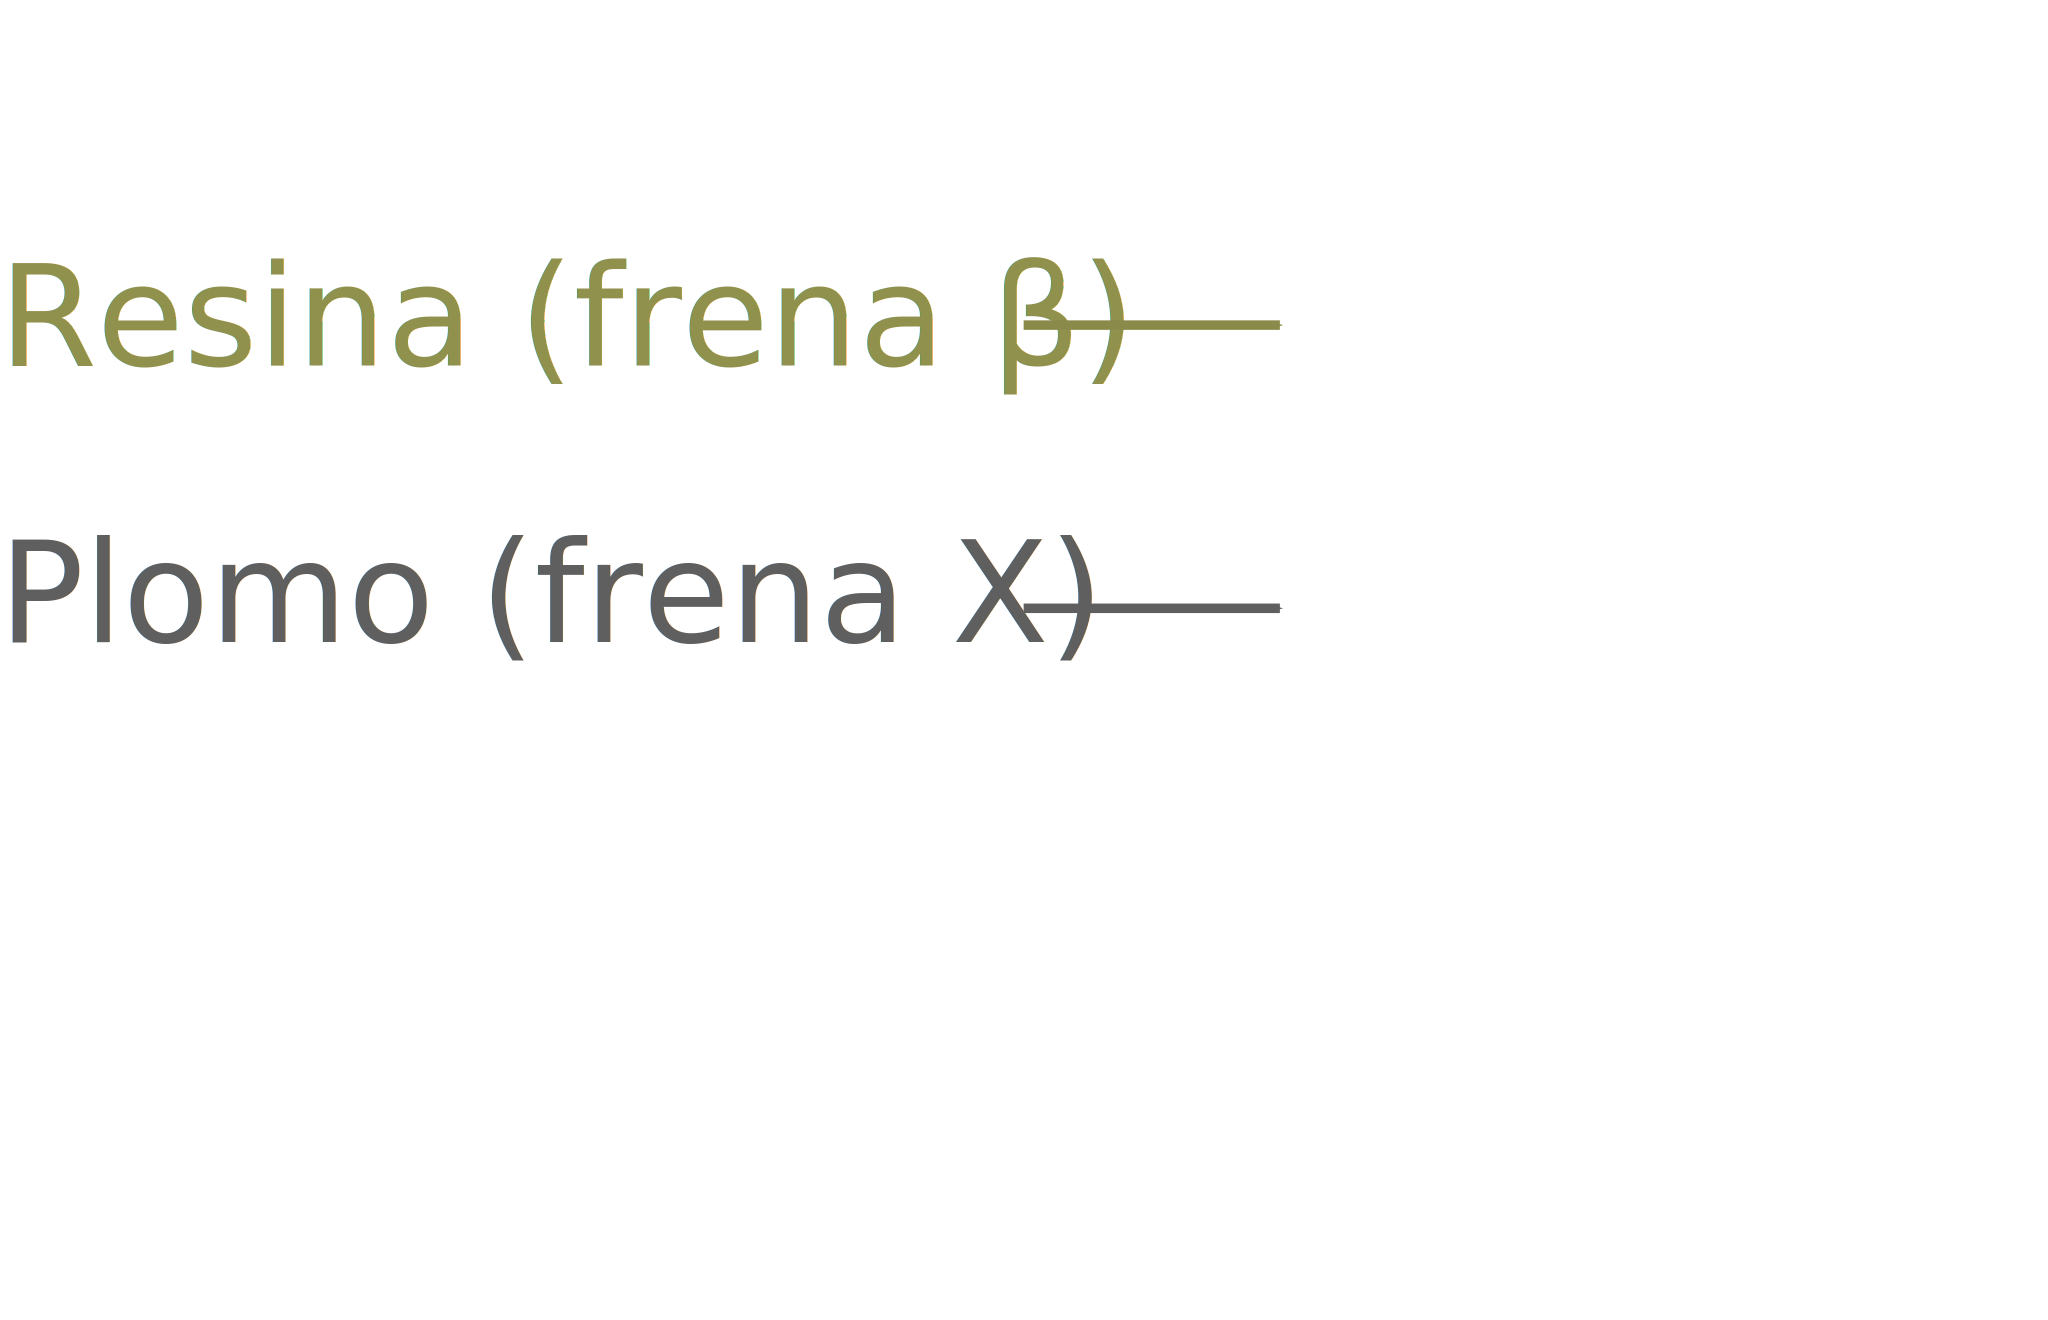
\includegraphics{figuras/poster/posicion_no.png}
        \caption{Posición segura.}
        \label{fig:posicionno}
    \end{subfigure}
    \hspace{5mm}
    \begin{subfigure}[b]{.45\textwidth}
        \includegraphics{figuras/poster/posicion_si.png}
        \caption{Posición para irradiar.}
        \label{fig:posicionsi}
    \end{subfigure}
    \caption{Posiciones de la pieza giratoria.}
    \label{fig:posicionespieza}
\end{figure}
\subsection{Construcción}
\subsubsection{Paredes}
Cubrimos ambos extremos de la cavidad con discos de acrílico
de \SI{10}{\milli\meter} de espesor y \SI{90}{\milli\meter} de diámetro.

Para los laterales consideramos moldear tubos de parafina o acrílico
debido a la dificultad de conseguir tubos de PVC con paredes de
\SI{10}{\milli\meter}.
Finalmente optamos por usar un tubo interior y uno exterior de PVC,
y rellenar el espacio intermedio con acrílico.
\subsubsection{Pieza giratoria}
La pieza giratoria está hecha de plomo fundido y luego mecanizado
(\figref{fig:construccion_mariposa}).
\fig{construccion_mariposa}{figuras/irradiador/construccion_mariposa.pdf}
{Pasos para la fabricación de la pieza giratoria de plomo.
El torneado requiere un lugar de donde agarrar a la pieza,
que luego cortamos.}
Para la fundición recurrimos a Abraham Murillo en la 
Escuela Técnica Nº 33 Fundicion Maestranza del Plumerillo. 
Allí tornearon una forma de madera con las dimensiones aproximadas de la pieza final.
La hicimos un poco más grande que las dimensiones finales tomando en cuenta
\begin{itemize}
    \item la contracción del plomo al enfriarse, y
    \item el margen de material extra necesario para tornear.
\end{itemize}
Rodeamos esta forma con tierra apisonada para crear un molde.
El mismo cuenta con un tubo para verter el metal fundido 
y un agujero para ventear gases
(\figref{fig:moldeplomo}).
\fig{moldeplomo}{figuras/irradiador/molde_plomo.pdf}
{Corte del molde usado para fundir la pieza giratoria de plomo.
Está hecho de tierra apisonada alrededor de una forma de madera.
Vertimos el plomo fundido por el tubo de la derecha.
El agujero superior sirve para ventear gases.}
La pieza que sale de este proceso tiene una superficie rugosa
debido a los granos de la tierra usada para el molde.
Para darle una terminación lisa y las dimensiones exactas que necesitamos,
recurrimos a Eriel Fernandez del taller mecánico de FIUBA.
La idea original era darle forma esférica,
pero descartamos esta idea debido a la dificultad
de tornear una esfera en un torno manual.
En cambio, optamos por una forma fácil de tornear
pero que obture lo más posible la cavidad del irradiador 
y pueda girar dentro de la misma
(\figref{fig:torneo_simple}).
\fig{torneo_simple}{figuras/irradiador/torneo_simple.pdf}
{Elegimos una forma simple de tornear que obture lo más posible 
la cavidad del irradiador y pueda girar en su interior.
Para eso nos aseguramos de que las esquinas no se salgan de un círculo
con el diámetro interior de la cavidad.}
Las dimensiones finales están en la \figref{fig:torneo}.
La blandez del plomo demandó un torneado cuidadoso a bajas revoluciones.
\fig{torneo}{figuras/irradiador/torneo.pdf}
{Corte lateral de la pieza giratoria de plomo luego del torneado
(dimensiones en mm).}
\subsubsection{Mochila de la fuente}
La fuente va colocada en una pieza de plástico.
Si bien la fuente cuenta con un agujero roscado,
fijarla con un tornillo requiriría manipularla de cerca,
exponiendo las manos a radiación durante cierto tiempo.
Por eso decidimos montarla en un bolsillo donde se puede 
rápidamente dejar caer la fuente,
minimizando la exposición del que realice la tarea.

Quisimos asegurarnos de que el plástico frene todos los electrones antes de llegar a
la pieza de plomo. 
Para eso le dimos una forma redonda que cubra lo más posible al plomo,
con la restricción de que pueda girar en la cavidad.

Debido a la dificultad de moldear esta forma (redonda y con una cavidad)
en resina, recurrimos a Iván G. Pollitzer y el 
Laboratorio Abierto de Electrónica de FIUBA.
Iván nos guió en el diseño de una pieza impresa en 3D en ABS.
Esta pieza consiste en dos partes impresas por separado
(\figref{fig:blender}),
\fig{blender}{figuras/irradiador/blender_small.png}
{Las dos partes que imprimimos en 3D en ABS y pegamos para formar la montura de
    la fuente.
Entre las dos partes queda un bolsillo donde se coloca la fuente.}
que luego rellenamos de acrílico y unimos.

Unimos la mochila de plástico a la pieza de plomo usando tornillos sin cabeza,
agujereando y roscando ambas piezas.
\subsection{Cálculos de protección}
\subsubsection{Frenado $\beta$}
% FIXME: repetido, todo esto está en la sección anterior
Usamos PVC para el frenado de electrones, porque está disponible en tubos
del tamaño requerido.
Tiene baja eficiencia radiativa y el rango de nuestros electrones más
energéticos en PVC es inferior a \SI{1}{\centi\meter}.
Por las mismas razones construimos las tapas del cilindro con discos de
acrílico de \SI{1}{\centi\meter} de espesor,
pegados a las tapas de plomo.
La mochila donde montamos la fuente consiste de plástico ABS 
extruído en una impresora 3D en el LABi.
Esto requirió separar el modelo inicial en dos partes que fueron pegadas y
terminadas con herramientas manuales.
%
\subsubsection{Cálculos de radiación de frenado}
Las partículas $\beta$ de la fuente empiezan a frenarse en el plástico,
donde producen radiación X de frenado.
Estimamos su magnitud partiendo del espectro de energía de los
electrones emitidos por la fuente.
Dado que está en equilibrio secular 
(misma actividad de \Strontium y de \Yttrium),
sumamos sus espectros provenientes de 
Radiological Toolbox\cite{eckerman2006radiological}
y normalizamos a la actividad nominal de la fuente, \SI{100}{\milli\curie}
(\figref{fig:actividadsr90}).
\fig{actividadsr90}{figuras/irradiador/actividad.pdf}
{Espectro de electrones provenientes de una fuente de
\Strontium con actividad \SI{100}{\milli\curie}\cite{eckerman_icrp_2007}.}
Luego calculamos el espectro de bremsstrahlung integrando la \equref{eq:kramers}
(\figref{fig:espectrox}).
\fig{espectrox}{figuras/irradiador/espectrox.pdf}
{Espectro de bremsstrahlung calculado en la cara exterior del PVC.}
%
\subsubsection{Atenuación de rayos X en el plomo}
Aplicamos la \equref{eq:absorcionx} 
usando tasas de absorción en plomo tabuladas por NIST\cite{xraycoef},
resultando en el espectro atenuado de la \figref{fig:xatenuado}
\fig{xatenuado}{figuras/irradiador/xatenuado.pdf}
{Espectro de rayos X calculado en la cara exterior del irradiador.}
% TODO: tasa de dosis final según distancia, comparar con mediciones
%
%
\subsubsection{Cálculos Monte-Carlo de fuente de \Strontium}
La fuente de \Strontium  emite electrones con un espectro amplio de
energías (\figref{fig:actividadsr90}).
Este consiste en la suma del espectro de emisión de \Strontium
y el de \Yttrium.
Simulamos un haz de electrones con este espectro incidiendo normalmente sobre
tejido blando, registrando la energía que depositan en función de la
profundidad (\figref{fig:deposicionsr90}).
\fig{deposicionsr90}{figuras/montecarlo/deposicion_sr90.pdf}
{Energía depositada en tejido blando en función de la distancia,
promediando entre electrones provenientes de una fuente de \Strontium.}
Así ajustamos una potencia de frenado de masa promedio $S/\rho$ (\figref{fig:stoppingsr90})
\fig{stoppingsr90}{figuras/montecarlo/stopping_sr90.pdf}
{Potencia de frenado promedio del tejido blando para electrones provenientes de
una fuente de \Strontium.
La cruz marca que a una profundidad de \SI{0.35}{\milli\meter} la tasa de dosis 
coincide con la tabulada en \cite{delacroix_radionuclide_2002}.}
que permite calcular tasa de dosis superficial mediante
\begin{align*}
    \dot D &= \frac{AS/\rho}{4\pi r^2}
\end{align*}
con $A=\SI{100}{\milli\curie}$ la actividad de la fuente.
La tasa de dosis calculada de este modo es comparable con la tabulada en
\cite{delacroix_radionuclide_2002} si se promedia hasta una profundidad de
\SI{.35}{\milli\meter}.
Esto sirve como verificación de que nuestras simulaciones Monte-Carlo producen
valores compatibles con los que se encuentran en la literatura.
\subsubsection{Cálculos Monte-Carlo del irradiador}
Buscamos una cota superior de la tasa de dosis fuera del irradiador.
Esto brinda la mayor confianza en que su operación no es peligrosa.
Ya que el espesor del plomo es de varias longitudes características de
atenuación ($1/\mu$),
sólo pasa una fracción muy pequeña de la radiación inicial.
Por lo tanto, hay que simular la emisión de 
muchos electrones de la fuente de \Strontium
para que llegue una cantidad apreciable de radiación a la cara exterior.
Así podemos estimar de forma precisa la tasa de dosis.

Una forma de reducir el tiempo de CPU necesario para simulaciones
es usar reducción de la varianza\cite{dressel_geometrical_2003}.
Esta es una técnica para cálculos Monte Carlo que introduce un sesgo en la
evolución de la partícula.
Por ejemplo, podemos aumentar la probabilidad de que una partícula atraviese
el plomo sin interactuar, en vez de scatterear.
Llevando la cuenta de cuan improbable es la historia de la partícula,
le damos un peso menor en la estadística final.
Esto concentra la simulación en darnos muchos eventos que nos interesan
(lo cual reduce la varianza de la estimación),
minimizando la capacidad de procesamiento necesaria.

Dada la dificultad de implementar reducción de la varianza en Geant4,
optamos por acelerar el cálculo simplificando la geometría.
Simulamos un irradiador con simetría esférica,
que consiste en un cascarón de \SI{10}{\milli\meter} de acrílico rodeado por
\SI{36}{\milli\meter} de plomo (\figref{fig:corte_esferico}). 
\fig{corte_esferico}{figuras/irradiador/corte_esfera.png}
{Corte de la geometría simplificada que se usó para simular el irradiador en
Geant4.}
Toda partícula en el irradiador tiene que atravesar al menos ese espesor de
acrílico y plomo.
Por lo tanto, la dosis real va a ser aún menor a la simulada.
Dada la simetría del problema, no tenemos en cuenta la distribución en
$\theta$ y $\phi$ sino que promediamos sobre ambas variables.
Esto reduce enormemente el número de eventos necesarios para una buena
estimación de la tasa de dosis.
El resultado se ve en la \figref{fig:dosis_irradiador}.
\fig{dosis_irradiador}{figuras/montecarlo/dosis_irradiador.pdf}
{Perfil de deposición de energía en la simulación Monte-Carlo del irradiador.}
La dosis en la cara exterior del irradiador es
de \SI{20.3}{\milli\sievert} por año.
Este valor es aceptable si se tiene en cuenta que,
en condiciones reales, se toca el irradiador durante intervalos muy cortos
y el resto del tiempo se está a distancias mucho mayores.

\part{Diseño, fabricación y caracterización de dosímetros MOS no
convencionales}
\section{Dosímetro Active Pixel Sensor}
\fig{aps}{esquematicos/aps.pdf}{Esquemático del dosímetro APS}
El dosímetro APS tiene una estructura similar a un pixel del sensor de imagen
en una cámara digital. 
Su principio de funcionamiento es medir la carga generada por radiación en la zona desierta de
una juntura p-n.
Hay un nodo flotante del circuito que acumula esta carga,
conectado al cátodo del diodo (\figref{fig:aps}).
Antes de cada medición, se reinicia el circuito llevando este nodo a 
V$_{\text{DD}}$ mediante el transistor de reset M1.
La radiación que incide en la zona desierta de D1 interactúa con la red de
silicio, depositando energía a través de distintos procesos como scattering e
ionización (ver sección~\ref{sec:radiacion}).
Los fotones y electrones secundarios resultantes producen pares electrón-hueco,
que son arrastrados en direcciones opuestas por el campo eléctrico.
Los electrones se acumulan en el cátodo, descargándolo.
Luego de irradiar,
se mide su tensión a través de un par de seguidores M2 y M3.
Los mismos evitan que la medición de tensión modifique la carga en el nodo y
afecte al valor medido.
\subsection{Proceso de fabricación}
Fabricamos tanto el FG como el APS en el proceso XC06 de la empresa X-FAB
\cite{x-fab_0.6_2008}.
El mismo tiene una escala de \SI{0.6}{\micro\meter} y está diseñado para
tensiones de hasta \SI{5}{\volt}.
En su versión estándar, 
cuenta con 1 capa de polisilicio y 2 de metalización.
\subsection{Reset}
Cargamos el nodo flotante a través del drain de un MOSFET de canal P,
con el source conectado a \vdd.
Durante la irradiación llevamos su gate a \vdd, apagándolo.
Para resetear 
llevamos su gate a tierra.
Esto lo coloca en saturación,
cargando la juntura a corriente constante 
y aumentando $V_D$ linealmente hasta $V_t$.
Entonces entra en triodo y va reduciendo la corriente,
cargando asintóticamente hasta \vdd.
Esto permite llevarlo a $V_{dd}$,
mientras que una llave de tipo N sólo llegaría hasta $V_{dd}-V_{tn}$ antes de
apagarse.

El transistor de reset es de área mínima,
para que aporte la menor capacidad parásita posible al nodo flotante.
\subsection{Respuesta a partículas}
Cada partícula deposita una energía promedio que depende de su energía
cinética inicial\cite{berger_response_1969} (ver sección~\ref{montecarloaps}).
Una parte $E$ de esta energía se usa en la creación de pares electrón-hueco,
generando carga 
\begin{align*}
    Q &= \frac{qE}{E_i}
\end{align*}
con $q$ la carga del electrón y $E_i$ la energía de creación de pares,
\SI{3.62}{\electronvolt} en Si.
Esta carga aparece con signo negativo en el cátodo, descargándolo.
Su cambio de tensión
\begin{align*}
    \Delta V &= \frac{Q}{C}
\end{align*}
depende de la capacidad total del nodo $C$.
La misma tiene contribuciones de
\begin{itemize}
    \item juntura de D1,
    \item juntura Drain-Body de M1,
    \item Gate de M2, y
    \item conductores cercanos al nodo.
\end{itemize}
Estas capacidades pueden estimarse a partir de las especificaciones del 
proceso de fabricación,
que indican capacidad por unidad de área y por unidad de perímetro.
Para eso usamos herramientas de EDA (electronic design automation)
que realizan esta estimación automáticamente a partir de la geometría del
diseño (ver sección~\ref{section:diseno_aps}).
\subsection{Cálculos Monte-Carlo}
\label{montecarloaps}
El dosímetro APS detecta energía depositada 
en una región específica de un circuito integrado.
A fines de simularlo, 
simplificamos la geometría del die a tres regiones:
una superficie de SiO$_2$, un sustrato de Si 
y una zona sensible también de Si (\figref{fig:corteaps}).
\fig{corteaps}{figuras/aps/corte.pdf}
{Corte de la geometría usada para simular el APS en Geant4 (no a escala).}
Las dimensiones se extrajeron del diseño del APS 
y de las especificaciones del proceso de fabricación del chip.

Dado que el uso principal de Geant4 es en física de altas energías,
su configuración por defecto no permite simular electrones secundarios por
debajo de \SI{250}{\electronvolt}.
% DETAIL rango a 250eV ~ nm, qué me importa?
Para obtener precisión a escalas de distancia más chicas,
empleamos una lista de procesos compilada para simulaciones en
microelectrónica \cite{Raine201497}.
La misma simula con fidelidad electrones hasta \SI{16.7}{\electronvolt},
cuyo rango en Si es del orden de \SI{0.1}{\nano\meter}.

% FIXME falta este gráfico usando
% ../tesis/figuras/aps/deposicion1electron001.pdf y demás
Los resultados se encuentran en la \figref{fig:energia1electron}.
Se ve que los electrones menos energéticos tienden a frenarse por completo en
el detector, depositando toda su energía.
Los más energéticos, en cambio, depositan una fracción variable de su energía
total.
La energía depositada promedio se encuentra en la
\figref{fig:energiadepositadaaps}.
\fig{energiadepositadaaps}{../poster2015/aps_respuesta.pdf}
{Respuesta promedio a un electrón incidente,
en función de su energía inicial.
Se ve que los electrones menos energéticos se frenan completamente en el
detector.}
\subsection{Fuentes de ruido}
El APS se maneja con corrientes y variaciones de carga y tensión muy
pequeñas.
Por eso es crítico conocer los procesos que introducen ruido y su magnitud.
\subsubsection{Corriente de fuga de juntura p-n}
Al polarizar una juntura p-n en inversa, fluye una corriente de
pérdida\cite{sze_physics_2007} dada por
\begin{align*}
    I&=I_s(e^{\frac{qV}{\eta kT}}-1)
\end{align*}
con $V<0$ la tensión aplicada y $I_s$ y $\eta$ parámetros de fabricación de la
juntura.
El valor de $I$ fluctúa debido a la naturaleza discreta de los portadores que
atraviesan la barrera de energía de la juntura.
Esta fluctuación se denomina ruido \emph{shot}, una clase de ruido blanco:
su densidad espectral de potencia,
\begin{align*}
    i^2(f) &= 2q|I|,
\end{align*}
no varía con la frecuencia (hasta frecuencias muy altas).
\subsubsection{Fluctuaciones durante reset}
Durante el reset, se carga la juntura p-n hasta $V_{dd}$ a través de M1.
Cerca de la tensión final, M1 entra en modo triodo.
El ruido de Johnson\cite{baker_cmos_2010} del canal cargando la capacidad 
de juntura $C$ produce una varianza en la tensión final dada por
\begin{align*}
    \overline{v^2} &= \frac{kT}C.
\end{align*}
Esta incertidumbre en la tensión luego del reset se elimina usando 
la técnica Correlated Double Sampling\cite{white_characterization_1974}:
se mide tensión antes y después de la exposición a la radiación.
Al tomar la diferencia se elimina el ruido de reset,
presente en ambas por igual.
\subsection{Diseño del circuito}
\label{section:diseno_aps}
\begin{figure}[p]
    \centering
    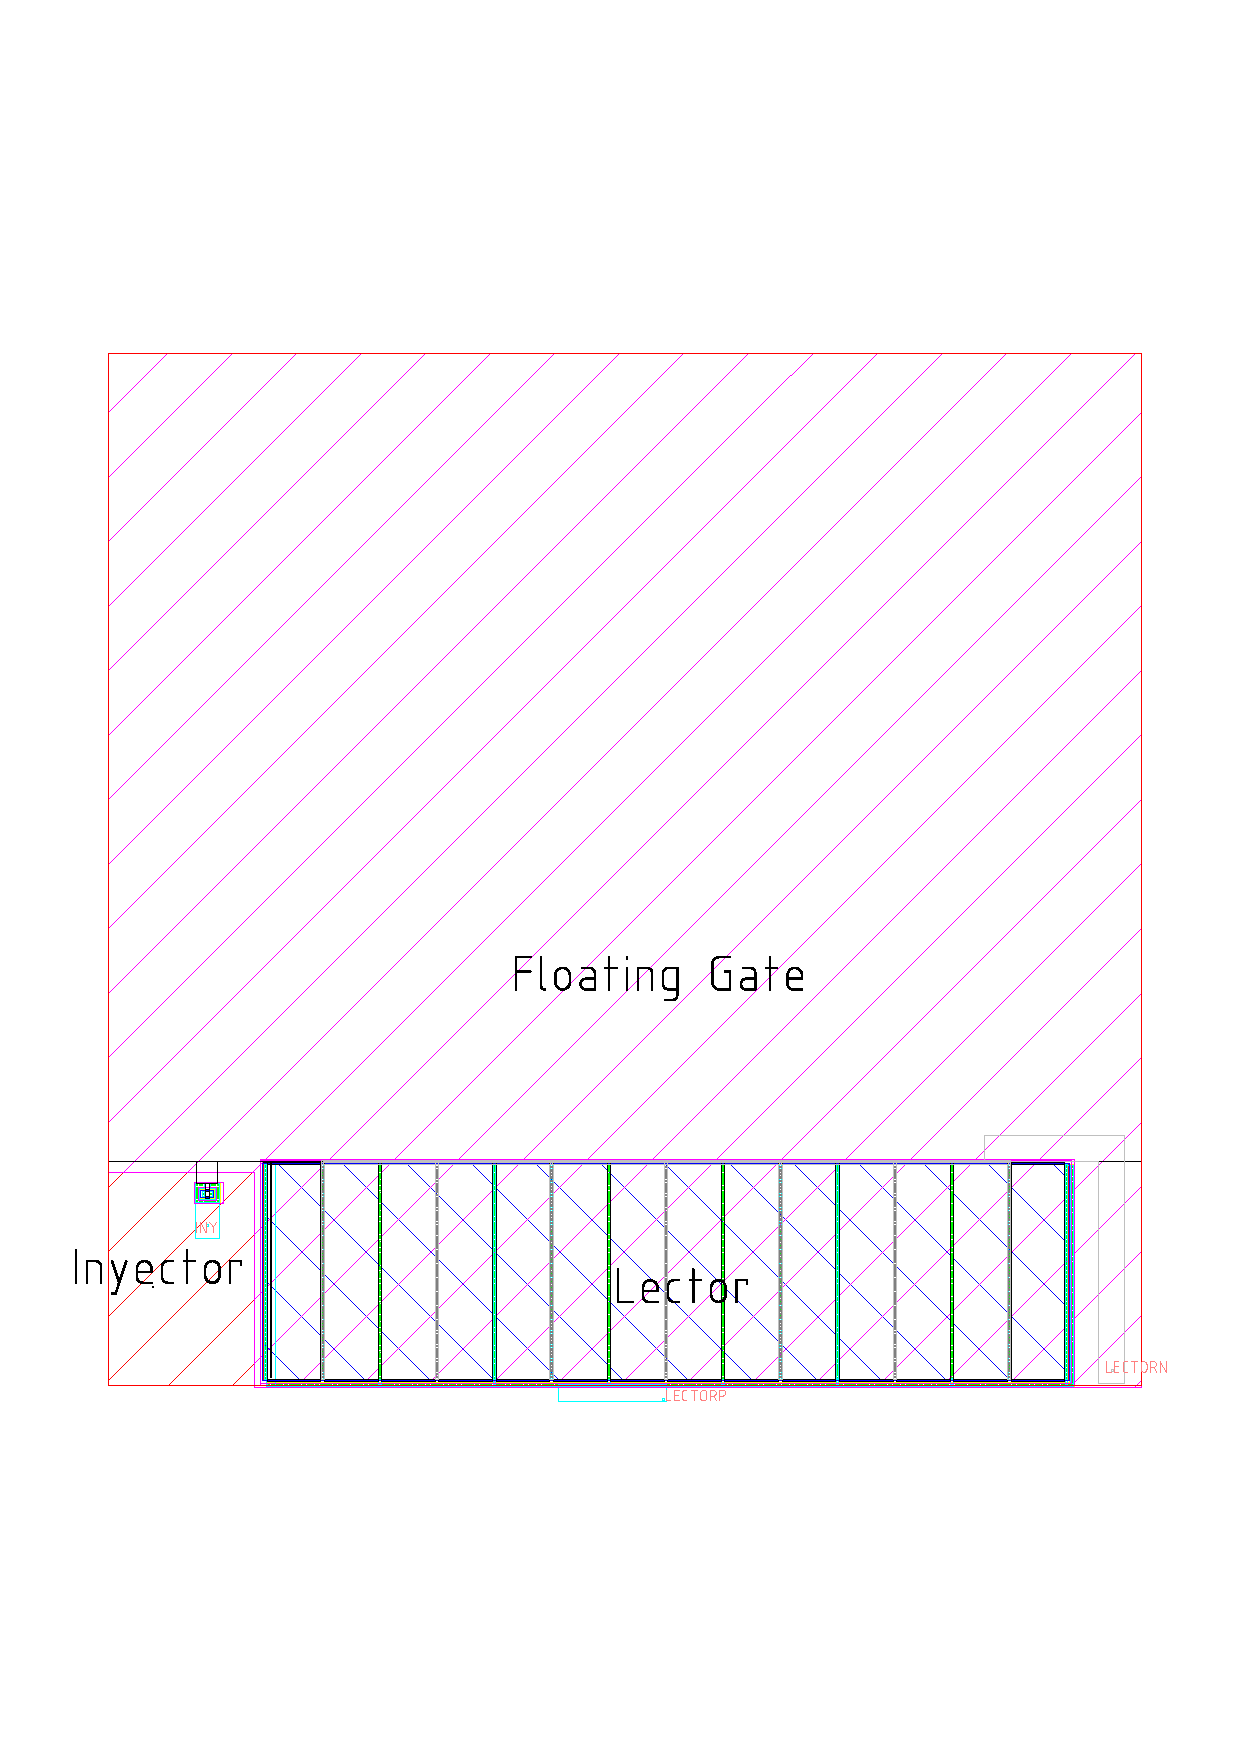
\includegraphics[width=\columnwidth]{figuras/aps/layout_hatch.pdf}
    \caption{Layout del dosímetro APS. 
    I1 es el espejo de corriente que polariza al primer seguidor M2.
    El transistor de reset M1 está conectado a un pad a través del
    circuito de protección de la \figref{fig:proteccion5v}.}
    \label{fig:layoutaps}
\end{figure}
\fig{proteccion5v}{figuras/aps/proteccion.pdf}
{Circuito de protección para la entrada de reset.
Los diodos sólo conducen si la tensión del pad excede \SI{5}{\volt} o
baja de \SI{0}{\volt}.
Esto evita que se polaricen en directa junturas del circuito que deben
permanecer en inversa (drain-bulk y source-bulk).}
La topología del circuito quedó determinada por la elección de construir un
dosímetro APS con un par de seguidores para su medición.
El paso siguiente en el diseño fue elegir los tamaños de los distintos
componentes para optimizar el desempeño del sensor (\figref{fig:falltime}).
\fig{falltime}{figuras/aps/falltime.pdf}
{Tiempo de respuesta simulado del buffer en función del W del transistor
final.}

Para una carga dada, la tensión sobre un capacitor es inversamente proporcional
a su capacidad.
Por lo tanto, maximizamos la señal producida por la radiación 
reduciendo las capacidades parásitas del cátodo de D1.
Para esto usamos transistores de área mínima en M1 y M2.
Restringimos el largo de las conexiones del cátodo,
y las mantuvimos alejadas de otros nodos.
Aplicamos software de Mentor de extracción de capacidades parásitas al layout
resultante, y obtuvimos una capacidad total en el cátodo de \SI{3.4}{\femto\farad}.
\begin{table}[h]
    \centering
    \caption{Dimensiones del diseño optimizadas para sensibilidad y tiempo de
    respuesta}
    \begin{tabular}{|c|c|}
        \hline
        Dispositivo&      Dimensiones\\
        \hline
D1&     \SI{4x4}{\micro\meter}\\
M1&     \SI{0.8x0.6}{\micro\meter}\\
M2&     \SI{0.8x0.6}{\micro\meter}\\
M3&     TODO\\
        \hline
    \end{tabular}
    \label{fig:areas}
\end{table}

Estas dimensiones se utilizaron tanto para la simulación del circuito en SPICE
como para los cálculos Monte-Carlo.
La combinación de estas dos herramientas nos da una sensibilidad esperada de 
\SI{7.1}{\volt\per\gray}.
\subsection{Medición}
Tomamos dos dies y los bondeamos a placas adaptadoras de TSSOP28,
un empaquetado de circuitos integrados de montaje superficial
(figuras~\ref{fig:bondeados1}, \ref{fig:bondeados2} y~\ref{fig:pinout}).
\fig{bondeados1}{figuras/aps/bondeados.jpg}
{Dies bondeados a placa adaptadora SMD.
Los zócalos tienen las patas cortocircuitadas para proteger al die de
descargas electrostáticas durante el transporte y almacenamiento.}
\figp{bondeados2}{figuras/aps/die.jpg}
{Detalle del die fabricado con los dosímetros APS y FG 
(arriba en la columna central)
y otros circuitos.}
\figp{pinout}{figuras/aps/pinout1.pdf}
{Layout del die entero con numeración de los pads bondeados}
\subsubsection{Descarga en oscuridad}
Primero medimos la respuesta del sensor sin luz ni radiación
(figuras~\ref{fig:oscuridad4} y~\ref{fig:oscuridad40}).
\fig{oscuridad4}{figuras/aps/oscuridad4.pdf}
{Curva de descarga en oscuridad del APS de 4x\SI{4}{\micro\meter}.
Resulta de resetear el APS y medir su tensión de salida en oscuridad.}
\fig{oscuridad40}{figuras/aps/oscuridad40.pdf}
{Curva de descarga en oscuridad del APS de 40x\SI{40}{\micro\meter}.
Resulta de resetear el APS y medir su tensión de salida en oscuridad.}
Esto nos muestra la descarga del diodo debido a la corriente de fuga en
inversa.

Se ve en ambas figuras la misma curva 
con escalas distintas de tiempo y de tensión.
Esta variación proviene tanto de las áreas distintas de los dos sensores
como del mismatching entre los seguidores.
Ya que éstos usan varios transistores de área mínima,
son particularmente sensibles a variaciones del proceso
(el mismo error absoluto en las dimensiones del canal produce un mayor error relativo).

% Descarga debería ser lineal
% https://books.google.com.ar/books?id=6Rg7AAAAQBAJ&lpg=PA289&ots=yO1HPv_N4E&dq=reverse%20biased%20diode%20%22discharge%20curve%22&hl=es&pg=PA290#v=onepage&q=reverse%20biased%20diode%20%22discharge%20curve%22&f=false
La forma de la curva proviene de la variación 
tanto de la corriente de fuga como de la capacidad del diodo.
Ambas dependen de la tensión aplicada,
debido a la variación del ancho de la zona desierta.
Al caer la tensión en inversa,
se vuelve más angosta.
Esto reduce su volúmen y por lo tanto 
la tasa de generación térmica de pares electrón-hueco.
Por otra parte,
su capacidad es inversamente proporcional a este ancho.
Ambos fenómenos reducen la tasa de descarga,
como se ve al final de ambas curvas.
%
\subsection{Iluminación con LED}
Medimos las curvas de descarga iluminando los dies con un LED,
variando su corriente para lograr distintas intensidades de iluminación
(figuras~\ref{fig:led4} y~\ref{fig:led40}).
\fig{led4}{figuras/aps/descarga_led_4.pdf}
{Curva de descarga iluminando con un LED el APS de 4x\SI{4}{\micro\meter}.
La corriente del LED aumenta de \SI{.1}{\milli\ampere} a la derecha hasta
\SI{10}{\milli\ampere} a la izquierda,
con 6 curvas por década.}
\fig{led40}{figuras/aps/descarga_led_40.pdf}
{Curva de descarga iluminando con un LED el APS de 40x\SI{40}{\micro\meter}.
La corriente del LED aumenta de \SI{.1}{\milli\ampere} a la derecha hasta
\SI{10}{\milli\ampere} a la izquierda,
con 6 curvas por década.}
Esto permite observar la compresión de la curva de descarga 
con el aumento de la radiación incidente.
\subsubsection{Ruido medido}
Establecimos que una medición con este dosímetro consiste en promediar 10
muestras de tensión.
Esto nos permite definir de manera precisa el ruido como la desviación estándar
de ese promedio.
Calculamos esa desviación estándar en base a las curvas medidas (figuras~\ref{fig:ruido4} 
y~\ref{fig:ruido40}).
\fig{ruido4}{figuras/aps/ruido4.pdf}{Ruido a la salida del APS de
    \SI{4x4}{\micro\meter}, calculado tomando diferencias entre muestras y
escalando para que represente el ruido en un promedio de 10 valores.}
\fig{ruido40}{figuras/aps/ruido40.pdf}{Ruido a la salida del APS de
    \SI{40x40}{\micro\meter}, calculado tomando diferencias entre muestras y
escalando para que represente el ruido en un promedio de 10 valores.}
Podemos convertir estos valores de ruido en dosis usando la sensibilidad
calculada.
Así llegamos a una resolución de \SI{2.0}{\milli\gray} y \SI{2.3}{\milli\gray}
para el APS de \SI{4x4}{\micro\meter} y \SI{40x40}{\micro\meter},
    respectivamente.
% TODO: completar con cálculos de sensibilidad/resolución y mediciones

\section{Dosímetro Floating Gate}
% TODO ?: diseño, cuentas, consideraciones
Los MOSFET con gate aislado o floating gate se usan comercialmente
en memorias no volátiles (Flash y EEPROM).
Se coloca cierta carga, 
cuyo valor representa uno o más bits de información, en el gate.
Luego se recupera la información midiendo la carga del gate
en base a las curvas IV del MOSFET.

El dosímetro FG se basa en un MOSFET con gate aislado.
Su modo de uso es primero resetearlo, dándole una carga inicial.
Desde el momento de reset, el dosímetro integra 
la dosis total que recibe sin necesidad de alimentación
(mientras no exceda una dosis máxima).
Por lo tanto es idóneo para seguimientos largos,
por ejemplo de un trabajador durante su turno.
%
\subsection{Principio de funcionamiento}
Su principio de funcionamiento es que la radiación que incide
en el óxido de compuerta tiende a descargar al FG.
Antes de irradiar,
se coloca carga en el gate mediante una corriente de túnel 
(\figref{fig:cargafg}).
\figp{cargafg}{figuras/fg/esquemainyeccion.pdf}
{ Inyección de carga en el FG a través de una corriente de túnel.
La tensión en el inyector produce un campo eléctrico en su óxido de gate,
que facilita una corriente de túnel Fowler-Nordheim.
La carga que pasa al FG prende el transistor lector.}
Esta carga altera la tensión de gate, prendiendo un transistor lector.

La radiación incidente produce pares electrón-hueco en el óxido
que rodea al floating gate, descargándolo
(\figref{fig:irradiacionfg}).
\figp{irradiacionfg}{figuras/fg/irradiacion.pdf}
{ Descarga del FG debido a pares electrón-hueco creados por
radiación.
Los huecos son atraídos a la carga negativa del FG y
se recombinan con la misma, descargándolo.}
Esto va apagando el lector,
reduciendo su corriente de drain si se aplica tensión drain-source constante
(\figref{fig:fg_vd_cte})
\figp{fg_vd_cte}{figuras/fg/lector_vd_cte.pdf}
{Variación de la corriente de drain del lector con la tensión de gate,
para distintos valores de $V_{sd}$.}
o aumentando su tensión drain-source si se aplica corriente de drain constante
(\figref{fig:fg_id_cte}).
\figp{fg_id_cte}{figuras/fg/lector_id_cte.pdf}
{Variación de la tensión de drain del lector con la tensión de gate,
para distintos valores de $I_d$.}
Calibrando estas cantidades contra la dosis recibida, 
el resultado es un dosímetro.
%
\subsection{Trabajos previos}
Thomsen\cite{thomsen_floating-gate_1991} produce un FG MOSFET
con un proceso estándar de \SI{2}{\micro\meter} con dos capas de polisilicio
a través del consorcio MOSIS\cite{noauthor_mosis_nodate}.
Su innovación consiste en usar túnel Fowler-Nordheim entre las capas de
polisilicio, en vez de usar electrones calientes. 
Así logra buenas corrientes de inyección para ambas polaridades,
aplicando tensiones de hasta \SI{20}{\volt}.

Tarr\cite{tarr_sensitive_2004} fabrica un FG en un proceso comercial CMOS
de \SI{1.5}{\micro\meter} con dos capas de polisilicio. 
Esto le permite aplicar la tensión de inyección 
(de hasta 40V) sin pasar por un MOS.
Usa un MOS lector apareado con otro MOS idéntico para compensar 
la variación con temperatura.
Como resultado obtiene una sensibilidad de \SI{3}{\milli\volt\per\rad}.

Cesari\cite{cesari_floating_2014} construye un dosímetro FG 
con un proceso de una sola capa de polisilicio.
Lo usa para estudiar el efecto de cargas y descargas repetidas
en el sensor.
En ambos casos controla la carga del FG eléctricamente,
aplicando tensiones de hasta \SI{18}{\volt}.

%
\subsection{Acoplamiento capacitivo}
% FIXME: mover a cargado FG
Ya que el FG está aislado,
su tensión es función de la carga que almacena 
y de la capacidad entre este y otros nodos del circuito.
Sumando la carga en cada capacidad se llega a la relación
\begin{align}
    Q_{FG} &= (C_R + C_W) V_{FG} + C_I (V_{FG}-V_I)
    \label{eq:ccoupling}
\end{align}
con $Q_{FG}$ la carga almacenada en el FG, $C_R$ la capacidad de gate del
lector, $C_W$ la capacidad del FG sobre el well del lector y $C_I$ la capacidad
de gate del inyector.
\subsection{Sensibilidad}
Para predecir la sensibilidad del dosímetro,
necesitamos un modelo simple de cómo la radiación
descarga al floating gate.

En principio, la radiación genera pares electrón-hueco
en todo el volúmen de óxido donde incide.
Esto sólo nos interesa cuando ocurre en el óxido que rodea al FG,
porque entonces esos pares electrón-hueco pueden descargarlo.
Por lo tanto, cada región de FG aporta una generación de carga
proporcional a su área $A$ y al espesor de óxido: $t$.

No podemos medir directamente la cantidad de carga en el floating gate.
Sólo podemos saberla indirectamente, a partir de la tensión de gate.
La relación entre carga y tensión es la capacitancia del FG.
Para cada región de FG, su capacitancia es proporcional al área $A$
e inversamente proporcional al espesor del óxido $t$
que la separa de lo que tiene debajo.

Por lo tanto, la sensibilidad 
(definida como derivada de la tensión respecto de la dosis)
es un cociente entre la carga generada por todo el óxido que rodea al FG
y la capacitancia del FG a otros nodos.
\begin{align}
    S = \deriv{V}{E} \propto \frac{\sum_i A_it_i}{\sum_j A_j/t_j}
    \label{eq:sensibilidad_fg}
\end{align},
con $A_i$ y $t_i$ las áreas y espesores de los óxidos que rodean al FG.
Tanto los óxidos de campo como de gate consisten de SiO$_2$,
de modo que la permitividad sale como constante.
Explorando esta ecuación, podemos optimizar el diseño del dosímetro
para maximizar su sensibilidad.
\subsection{Diseño}
El desempeño del dosímetro depende de cocientes
de capacidades entre FG y distintos nodos del circuito. 
Estos cocientes se reducen a relaciones entre las áreas del lector,
inyector y FG.
Debido a limitaciones del proceso de fabricación,
las áreas tienen un valor mínimo y varían de a pasos discretos.
Por otro lado, hay un área total máxima para el dosímetro.
Para elegir las dimensiones óptimas,
exploramos el espacio de soluciones mirando dos parámetros de calidad:
sensibilidad a la radiación, y eficiencia de inyección.

La ecuación~\ref{eq:sensibilidad_fg} dice que la sensibilidad se maximiza
asignando mayor área al óxido más grueso,
que es el óxido de campo entre FG y el well del lector.

Por otro lado,
la ecuación~\ref{eq:ccoupling} dice que la tensión de túnel $V_{FG}-V_I$
se maximiza, para un $V_I$ dado,
minimizando la relación $C_I/C_{FG}$.
Dado que hay un área mínima para el inyector,
es necesario aumentar las otras capacidades para reducir esa relación.

Exploramos el espacio de soluciones
graficando las curvas de nivel de ambos parámetros en función de dos variables
de diseño:
la relación área lector / área inyector,
y la relación área de well del lector / área inyector.
Esto se ve en las figuras~\ref{fig:sensibilidad_fg}
y~\ref{fig:eficiencia_inyeccion}.
\fig{sensibilidad_fg}{figuras/fg/sensibilidad.pdf}
{Sensibilidad del floating gate en función de la relación de áreas de 
inyector ($A_I$),
lector ($A_R$) 
y well del lector ($A_W$).}
\fig{eficiencia_inyeccion}{figuras/fg/inyeccion.pdf}
{Fracción de la tensión de inyección que cae en el óxido del inyector,
en función de la relación de áreas de 
inyector ($A_I$),
lector ($A_R$) 
y well del lector ($A_W$).}

Así llegamos a las dimensiones finales de cada región:
\begin{table}[h]
\centering
\begin{tabular}{|c|c|}
    Región   & Área (\SI{}{\micro\meter\squared})\\ \hline
Inyector & 4.32\\
Well     & 180000\\
Lector   & 35000
\end{tabular}
\end{table}
%
\subsection{Diseño físico (layout)}
%
\fig{layout_fg_todo}{figuras/gds/fg/small/poly_met.png}
{Layout del dosímetro completo, mostrando polisilicio y metalización.
El rectángulo superior de polisilicio está sobre nwell con óxido de campo,
y es la región principal de generación de carga por su óxido grueso.
Abajo a la izquierda está el inyector, 
el MOS de área mínima a través del cual se carga al FG.
Abajo a la derecha está el transistor lector,
armado con múltiples canales 
(varios MOSFET en paralelo que comparten difusiones source/drain).}
El layout (\figref{fig:layout_fg_todo}) se divide en 3 grandes regiones:
\begin{itemize}
    \item Floating Gate sobre óxido de campo y nwell,
    \item MOS inyector, y
    \item MOSFET lector.
\end{itemize}
El inyector es un MOS de área mínima con su propio nwell
(\figref{fig:layout_inyector}).
\fig{layout_inyector}{figuras/gds/fg/small/inyector.png}
{Layout del MOS inyector. Está rodeado por contactos a body (nwell).
Estos contactos y los de drain/source 
están cortocircuitados por la metalización (no visible).}
Esto permite conectar su drain, source y body a la terminal de inyección.

El lector es un MOSFET de $W=\SI{100}{\micro\meter}$ 
por $L=\SI{25}{\micro\meter}$ con 14 canales.
Esto significa que usa 14 MOSFET en paralelo,
que comparten difusiones source/drain. 
Esto se ve claramente en la metalización (\figref{fig:layout_fg_met}),
donde los source están conectados por debajo con M1 (la primera capa de metal)
y los drain por arriba con M2 (la segunda capa de metal).
\fig{layout_fg_met}{figuras/gds/fg/small/met1_met2.png}
{Metalización del FG.
A la izquierda, hay M1 (la primera capa de metal) 
cortocircuitando source, drain y body del MOS inyector.
A la derecha, hay M1 conectando por debajo los sources/body del MOSFET lector
y M2 conectando por arriba los drains.}
\subsection{Medición de la carga}
\fig{floatingcapacidades}{figuras/fgcapacidades/floatinggate2.pdf}{Modelo de
acoplamiento capacitivo en un MOSFET con floating gate.}
La tensión del floating gate controla el canal de un MOSFET
que llamamos lector o reader.
Para determinar esa tensión en función de la carga del FG,
usamos el acoplamiento capacitivo
\cita{pavan_floating_2004} 
entre floating gate y otros nodos, llegando a la ecuación
\begin{align*}
    V_{FG} &= \frac{C_I V_I + (C_R+C_W) V_R + Q}{C_I+C_R+C_W}
\end{align*}
con los términos ilustrados en la \figref{fig:floatingcapacidades}.

Durante la lectura se usa $V_I=V_R=0$.
En función de $V_{FG}$ y $V'_R$, la corriente del lector es
\begin{align*}
    I_R' &= \begin{cases}
        I_{D0} \left(\frac W L\right)_L
        \exp\left(\frac{V_{FG}-V_T}{nkT/q}\right)& V_{FG}>-V_T\\
        \beta_n\left(\frac W L\right)_L(V_{FG}+V_T+\frac{V'_R}2)V'_R &
        -V'_R-V_T<V_{FG}<-V_T\\
        \frac{\beta_n}2\left(\frac W L\right)_L(V_{FG}+V_T)^2 &
        -V'_R-V_T>V_{FG}.
    \end{cases}
\end{align*}
Estas ecuaciones nos indican que,
polarizando el lector con una tensión $V_{sd}$ pequeña
% FIXME: V_sd o V_r - V_{r'} ?
(usamos \SI{0.1}{\volt}),
estamos en la situación del medio y
la corriente de drain varía linealmente con $V_{FG}$
\subsection{Cargado del floating gate}
%
\subsubsection{Mecanismo de inyección}
Dado que el floating gate está aislado,
no es posible cargarlo o descargarlo con una fuente de tensión
como las placas de un capacitor normal.
La única forma de hacerle llegar carga es 
a través del aislante que lo rodea.

En condiciones normales, el aislante tiene muy pocos portadores.
Esto impide la conducción normal como en un metal.
Además, para espesores típicos de aislante, 
los electrones que están a uno y otro lado del mismo
no pueden tunelear a través de su barrera de potencial.
En consecuencia, el aislante presenta una resistencia alta.

Al aplicarle suficiente tensión,
el campo eléctrico en el aislante inclina la banda de conducción,
reduciendo el ancho de la barrera de potencial
(\figref{fig:fowlernordheim}).
Así aumenta la probabilidad de túnel, y en consecuencia la corriente.
Esto se denomina corriente de túnel
Fowler-Nordheim\cite{lenzlinger_fowlernordheim_1969}.
\fig{fowlernordheim}{figuras/fowlernordheim/fowlernordheim.pdf}
{Diagrama de bandas de la emisión de electrones del canal al gate de un MOS. 
El campo eléctrico en el óxido de gate reduce el ancho de la barrera de
potencial del óxido, facilitando el tuneleo.
Reproducido de \cite{lenzlinger_fowlernordheim_1969}}

Esta corriente se ajusta a una expresión del tipo
\begin{align*}
    J_{FN} &= AF_{ox}^2\exp(-B/F_{ox}).
\end{align*}
con $A$ y $B$ constantes de ajuste 
y $F_{ox}$ el campo eléctrico en el óxido.

Esto explica la corriente de gate que fluye en un MOS,
al aplicar tensión suficiente entre body y gate.
En nuestro caso, no podemos aplicar tensión directamente al gate
porque está completamente aislado.
Esto puede representarse como en la \figref{fig:cargadofg}.
\fig{cargadofg}{esquematicos/cargado_fg/cargado_fg.pdf}
{Esquemático del flujo de carga al floating gate 
a través del óxido del MOS inyector.
Al aplicar tensión al inyector,
parte de esta tensión cae sobre 
la capacidad de gate $C_I$ del MOS inyector 
y parte sobre la capacidad de well $C_W$ y del MOS lector $C_R$.
Minimizando $C_I$, se maximiza la tensión a través del inyector
y por lo tanto se logra la mayor corriente de túnel.}
La tensión se aplica al body de un MOS inyector,
cuyo gate es el FG.
Dándole al MOS inyector la menor área posible, 
reducimos su capacidad de gate.
Así la mayoría de la tensión de inyección cae a través de su óxido
y produce una corriente de túnel que carga al FG.

Dado que el FG tiene que prender un PMOS,
hay que darle una carga inicial negativa.
Mirando la \figref{fig:cargadofg},
una tensión negativa en el inyector
produce carga negativa en el FG.
Esta polarización pone al MOS inyector en acumulación,
de modo que la tensión gate-body cae principalmente 
en el óxido de gate (y muy poco en el silicio).

% FIXME: esto queda colgado
El campo en el óxido $F_{ox}$ está dado por 
\begin{align*}
    V_{FG}-V_I &= F_{ox}t_{ox}+\psi_s+V_{FB},
\end{align*}
con $V_{FB}=(\Phi_S-\Phi_M)/e$ 
y $\psi_s$ la caída de tensión sobre el Si del inyector,
que como ya dijimos es despreciable.
%
%Nuestro proceso de fabricación alcanza breakdown del
%óxido de gate al aplicar \SI{13}{\volt}.
%A esta tensión la densidad de corriente es
%\SI{.1}{\nano\ampere\per\micro\meter\squared}, cargando nuestro floating
%gate a razón de \SI{3.9}{\volt\per\second}.
% TODO: calcular / medir curva Fowler-Nordheim
\subsubsection{Experimental}
\fig{medicion_fg}{esquematicos/medicion_fg/medicion_fg.pdf}
{Setup experimental para inyectar corriente en el FG,
con todos los caminos de pérdidas relevantes.
La conexión del sustrato a la guarda de la fuente de corriente
anula la tensión a través del diodo sustrato-bulk del inyector.}
Cargamos el floating gate aplicando corriente constante
entre el inyector y el well del lector.
Durante la inyección,
cualquier conductancia parásita entre esos nodos 
va a llevarse parte de la corriente,
reduciendo la carga inyectada.
Al mismo tiempo, parte de la carga proporcionada
va a cargar las capacidades del sistema.
Si aplicamos una corriente pequeña
(para cambiar lentamente la carga del FG),
el setup de inyección está la mayoría del tiempo cargando estas capacidades
hasta que se alcanza la tensión necesaria para el tuneleo de inyector a FG.

Usamos la guarda de la fuente de corriente para eliminar algunos caminos de pérdida
(\figref{fig:medicion_fg}).
Conectándola al sustrato evitamos la corriente en inversa del diodo de bulk
del inyector.
Ya que el inyector está bondeado al pin siguiente al well del lector,
no es posible interponer una guarda entre ellos para evitar pérdidas en el PCB.
\subsubsection{Curvas de carga y descarga}
La tensión del inyector (figuras~\ref{fig:descarga_inyector}
y~\ref{fig:carga_inyector})
varía linealmente mientras se carga la capacidad de los cables a corriente
constante.
Cuando alcanza una diferencia de potencial suficiente respecto del FG,
la corriente de túnel crece rápidamente y frena el crecimiento de la tensión.
Las curvas IV (figuras~\ref{fig:descarga_iv}
y~\ref{fig:carga_iv}) saturan a corrientes cada vez más grandes/chicas,
confirmando la variación de tensión del FG entre cada tramo
de inyección.
\fig{descarga_inyector}{figuras/fg/21a29dip_inyector.pdf}
{Descarga del FG midiendo tensión del inyector (línea punteada) y
corriente de drain del lector (línea sólida) a
$V_{sd}$=\SI{100}{\milli\volt}.
Esta corriente de drain es una indicación directa 
de la cantidad de carga en el FG.}
\fig{descarga_iv}{figuras/fg/21a29dip_iv.pdf}
{Curvas IV del lector medidas entre tramos de la descarga
    de la \figref{fig:descarga_inyector}.}
\fig{carga_inyector}{figuras/fg/12a21dip_inyector.pdf}
{Carga del FG midiendo tensión del inyector (línea punteada) y
corriente de drain (línea sólida) a
$V_{sd}$=\SI{100}{\milli\volt}.}
\fig{carga_iv}{figuras/fg/12a21dip_iv.pdf}
{Curvas IV del lector medidas entre tramos de la carga.}
\subsection{Irradiación con \Strontium}
Expusimos el dosímetro,
previamente cargado,
a una fuente de \Strontium.
La \figref{fig:irradiacionfg_respuesta} muestra que la corriente responde de
manera casi lineal a la dosis.
La variación de la sensibilidad se ve con más detalle en la
\figref{fig:irradiacionfg_sensibilidad}.
\fig{irradiacionfg_respuesta}{figuras/fg/irradiacion_corriente.pdf}
{Corriente del lector del FG polarizado con
    $V_{sd}$=\SI{100}{\milli\volt} en función de la dosis recibida.
    % TODO: mover al texto?
    % TODO: originalmente decia ``sensibilidad inicial'', cual es la correcta?
La corriente calculada parte de la corriente inicial extraída de la
medición.}
\fig{irradiacionfg_sensibilidad}{figuras/fg/irradiacion_sensibilidad.pdf}
{Sensibilidad del FG polarizado con
    $V_{sd}$=\SI{100}{\milli\volt} en función de la dosis recibida.
}
% TODO: tomar valor absoluto para aclarar que la sensibilidad aumenta
La sensibilidad cambia con la dosis debido a dos fenómenos opuestos.
\begin{itemize}
    \item A medida que se descarga el floating gate, disminuye el 
        campo eléctrico en el óxido y baja el yield de generación de pares 
        electrón-hueco.
    \item Al reducirse la corriente, crece $\frac{dI_D}{dV_G}$ 
        (\figref{fig:didv}) y esto aumenta la sensibilidad.
\end{itemize}
Se ve en las mediciones un crecimiento de la sensibilidad que se aplana al
alzanzar \SI{50}{\Gray}.
\fig{didv}{figuras/fg/didv.pdf}
{La pendiente de la curva $I_D(V_G)$ del lector aumenta a medida que $I_D$ cae,
incrementando la sensibilidad del FG.
Esta curva fue simulada con modelos provistos por el foundry,
debido a que la compuerta del dispositivo fabricado es inaccesible para
mediciones.}
\subsection{Corriente de ruido}
Establecimos que una medición con este dosímetro consiste en promediar 10
muestras de corriente.
Así podemos definir el ruido como la desviación estándar de este promedio.
Medimos la corriente del lector en ausencia de radiación y
tomamos la diferencia entre muestras sucesivas para eliminar derivas
(\figref{fig:ruidofg}).
Esto resulta en una desviación estándar
$\sigma=$ \SI{27}{\nano\ampere},
correspondiente a una dosis de \SI{4}{\milli\gray}.
\fig{ruidofg}{figuras/fg/ruido.pdf}{Diferencia entre
mediciones sucesivas de corriente del lector, escaladas para representar el
ruido en promedios de 10 muestras.}
% TODO: otra estimación de ruido/resolución

\part{Discusión y conclusiones}
\section{Discussion}
\subsection{Use of standard CMOS processes}
The main difficulty in designing dosimeters in standard CMOS processes
is that these processes are not designed for this purpose.
The sensitivity has a subtle dependence on the geometry and doping of the
various circuit structures.
For ordinary analog circuits, it is enough for the foundry to control and inform the designer about
certain device parameters: threshold voltages, saturation currents, capacitances, leakage currents, etc.
Although we succeeded in designing dosimeters based on this limited information,
it would be ideal to optimize the design using more detailed 
(possibly confidential) process information.
\subsection{Biasing Monte-Carlo simulations}
The irradiator Monte-Carlo simulations used a spherically symmetrical model
in order to minimize runtime while providing a reasonable wort-case dose estimate.
The problem with this kind of simulation is that we are only interested in 
the small fraction of particles which escape the irradiator,
while the simulator wastes time tracking those which never escape.
It would be valuable for further works to use simulation biasing.
This is a technique used in radiation protection,
which allows for simulation time to be focused on certain outcomes.
This is done by biasing the generation of random numbers so that interesting outcomes
(e.g. particles which escape) are more likely.
In the end, the results are corrected to reflect how unlikely they are in reality.
\subsection{ESD protection structures}
Measurements were limited by the fragility of the samples,
which probably suffered from ESD (electrostatic discharge) damage.
Although protection structures were used in the APS reset inputs,
future designs should look into additional protections.
In particular, there should be a way to protect the FG injector
while allowing it to reach the elevated injection voltages.
\subsection{Leakage-minimizing layout}
The dosimeters were not laid out with leakage current in mind.
Both of them are sensitive to small leakage currents, whether before or during irradiation.
Future iterations should explore using guard rings or possibly changes to the circuit
which keep leakage currents under control.
\subsection{APS discharge curves}
The small and large APS have very different discharge curves.
This discrepancy has no immediate explanation, and neither does the unusual shape of the curves.
Although the LED measurements confirm that the APS are sensitive to incoming light,
it would be desirable to understand the exact shape of these curves.
This would allow us to better understand the discharge phenomena and build a more robust dosimeter.
\subsection{Adding a control gate to the FG dosimeter}
It is possible to reach a deeper understanding of the FG dosimeter by adding an externally accessible gate.
This can be done by routing metal over the FG, creating a capacitor.
It would allow for new ways of characterizing the device,
for example by measuring the shift in Vt as seen from the control gate.
\subsection{Anomalous variation of the FG sensitivity}
It was not possible to achieve a close fit to the measured FG sensitivity.
This suggests that the model we tried to fit is not capturing all relevant processes
such as interface state creation or oxide charge capture.
We can still calibrate the sensor using the empirical curve.
Nevertheless, it would be better to look for designs which minimize
the influence of processes which are outside our control.
This would lead to a dosimeter which is less sensitive to process variations.
% layout con más cuidado, faltaron guardas

\section{Conclusiones}
En este trabajo explicamos las carácterísticas generales, 
el principio de funcionamiento, 
la forma de diseño y el resultado de las mediciones de dos dosímetros.
Ambos diseños fueron elegidos porque representan una tendencia no sólo de
la dosimetría sino de toda la microelectrónica:
la integración de circuitos especializados en procesos CMOS.

Dimos un repaso de la física necesaria para entender el principio de
funcionamiento de ambos dosímetros, centrándonos en la operación del transistor
MOS. Para esto cubrimos sus regiones de operación y resumimos los principales
efectos de la radiación.

Tanto en el diseño del irradiador como del dosímetro APS presentamos los
cálculos Monte-Carlo con los que contrastamos las dosis calculadas
analíticamente. En ambos casos detallamos la geometría simplificada que usamos
para la simulación, ya sea para minimizar el tiempo de cálculo (caso del
irradiador) o por falta de información acerca de las dimensiones (caso del
APS).

Para cada circuito partimos de la topología elegida explicando los valores a
elegir, y las medidas de desempeño que buscamos maximizar. Para eso mostramos
los cálculos y simulaciones que guiaron el proceso de diseño.

Finalmente presentamos las mediciones realizadas sobre los dosímetros
fabricados. Extrajimos un subconjunto de las medidas de desempeño anteriores y
las comparamos con los valores esperados en base a la simulación del diseño
final.

En la discusión evaluamos en detalle los aspectos positivos y negativos de todo
el trabajo y aquellos cambios, mejoras o profundizaciones que quedan abiertos
para trabajos futuros.


%\bibliographystyle{ieeetr}
%\bibliography{bibliografia}
\printbibliography

\end{document}
